\documentclass[11pt,letterpaper]{article}
\usepackage[T1]{fontenc}
\usepackage[utf8]{inputenc}
\usepackage{lmodern}
\usepackage[margin=1in,headheight=15pt]{geometry}
\usepackage{amsmath,amssymb,amsthm,mathtools}
\usepackage{microtype,booktabs,longtable,tabularx,array}
\usepackage[dvipsnames]{xcolor}
\usepackage{graphicx,float,fancyhdr,enumitem,listings}
\usepackage[numbers,sort&compress]{natbib}
\usepackage{xurl}
\usepackage{hyperref}
\definecolor{ink}{HTML}{17324D}
\definecolor{accent}{HTML}{167D9A}
\definecolor{light}{HTML}{F2F5F8}
\hypersetup{colorlinks=true,linkcolor=ink,citecolor=accent,urlcolor=accent,
 pdftitle={Topology in Three Records and Bidirectional Survivor Transfer},
 pdfauthor={Research continuation prepared for Vladimir Reshetnikov}}
\pagestyle{fancy}
\fancyhf{}
\fancyhead[L]{\small\color{ink}Exact compression for unknot recognition}
\fancyhead[R]{\small\color{ink}Research continuation}
\fancyfoot[C]{\thepage}
\setlength{\parskip}{0.35em}
\setlength{\parindent}{1.3em}
\setlist{topsep=4pt,itemsep=3pt}
\setcounter{tocdepth}{2}
\newtheorem{theorem}{Theorem}[section]
\newtheorem{lemma}[theorem]{Lemma}
\newtheorem{proposition}[theorem]{Proposition}
\newtheorem{corollary}[theorem]{Corollary}
\theoremstyle{definition}
\newtheorem{definition}[theorem]{Definition}
\newtheorem{researchquestion}{Research question}[section]
\theoremstyle{remark}
\newtheorem{remark}[theorem]{Remark}
\newcommand{\F}{\mathbb F_2}
\newcommand{\Hom}{\operatorname{Hom}}
\newcommand{\im}{\operatorname{im}}
\newcommand{\rank}{\operatorname{rank}}
\newcommand{\code}[1]{\texttt{\detokenize{#1}}}
\lstset{basicstyle=\ttfamily\small,columns=fullflexible,breaklines=true,
 backgroundcolor=\color{light},frame=single,rulecolor=\color{light},
 keepspaces=true,showstringspaces=false,xleftmargin=5pt,xrightmargin=5pt}
\begin{document}
\hypersetup{pageanchor=false}
\begin{titlepage}
\vspace*{0.6in}
{\large\color{accent}\sffamily PROVEIT / TOPOLOGY / RESEARCH CONTINUATION\par}
\vspace{0.32in}
{\Huge\bfseries\color{ink}Topology in Three Records\par}
\vspace{0.1in}
{\LARGE\bfseries\color{ink}and Bidirectional Survivor Transfer\par}
\vspace{0.27in}
{\Large Two exact compression kernels for unknot recognition\par}
\vspace{0.4in}
{\large Prepared for Vladimir Reshetnikov\par}
{\large 8 October 2026\par}
\vspace{0.35in}
\noindent\textcolor{accent}{\rule{\textwidth}{1.2pt}}
\vspace{0.2in}
\begin{abstract}
We develop two exact compression results motivated by the current
\emph{ProveIt} unknot-recognition implementation. First, a finite covering
of a connected bordered surface whose fibre monodromy has the form
$x\mapsto\pm x+a\pmod W$ has at most three families of connected
components, isomorphic as covers within each family. We give explicit
formulas for their multiplicities, orientability, genera, and every
boundary covering degree; the bound is sharp even for orientable bases.
The arithmetic depends polynomially on $\log W$ and supports marked
component and boundary queries without expanding the sheets.

Second, we express a quantum-graded scalar contraction's transferred
differential as a typed acyclic path sum. We prove that only paths between
surviving objects need be retained, and that each resulting component may
be evaluated from either end. This gives exact direction-sensitive work
bounds and graded families with quadratic versus linear transfer work.
A further implementation contracts the scalar graph component by
component and uses sparse index columns, avoiding artificial quadratic
bit storage on disconnected scalar blocks. Combined with Boolean
reachability, it gives a complete near-linear reduction stage on a fixed
coefficient algebra where inherited forward transfer alone takes
quadratic work.

The package supplies complete proofs, optional scanner integration,
independent contraction and topology checks, source snapshots, and paired
benchmarks including negative results. The unrestricted
$n^{O(\log n)}$ goal remains unresolved: the geometric kernel requires a
certified covering presentation, and the scanner still lacks a universal
bound on intermediate object multiplicities. These limitations are stated
as precise remaining mathematical obligations.
\end{abstract}
\vfill
\noindent\small Repository baseline:
\href{https://github.com/VladimirReshetnikov/ProveIt/commit/9cec5275f2d2113d0a784cedf156460829b61489}{\texttt{9cec5275f2d2113d0a784cedf156460829b61489}}.\\
The mathematical proofs are written out; the computational checks are
finite verification, not a Lean formalization or a claim of general
quasi-polynomial recognition.
\end{titlepage}
\pagenumbering{roman}
\hypersetup{pageanchor=true}
\tableofcontents
\clearpage
\pagenumbering{arabic}
\section{Problem, baseline, and precise contributions}
\label{sec:scope}

The computational objective is to decide whether a planar diagram with
$n$ crossings represents the unknot, with a proved running time of
$n^{O(\log n)}$. The current project has a sound exact recognition
pipeline with several polynomial or restricted-input front ends and
a Bar--Natan scanning implementation of Khovanov homology over $\F$.
The unrestricted Khovanov backend is complete; explicit resource limits
may return \texttt{UNKNOWN}. Its unrestricted worst-case bound is
exponential. This continuation
studies representations that remove two specific kinds of unnecessary
expansion: repeated geometric sheets and repeated algebraic transfer
paths.

\subsection{What was already established}

The audit is anchored to the repository snapshot dated 8 October 2026
at commit \texttt{9cec5275f2d2}, whose full identifier is on the title page
\cite{ProveItSnapshot2026}. The maintained implementation and its tests
are the software baseline. The
following relevant developments precede this report.

\begin{center}
\small
\begin{tabularx}{\textwidth}{@{}p{0.17\textwidth}X@{}}
\toprule
Prior work & Result used or respected here \\
\midrule
Reports 07--09 & Structural certificates, exact component sharing,
specialized braid recognition, certified factorization, and sparse
algebraic filters. \\
Reports 10--12 & Component cobordism contraction, restart accounting,
twist compression, and succinct block cancellation. \\
Report 13 & Exact prescribed homological windows with guard degrees and
support-aware allocation. \\
Reports 14--15 & Continuation quotients, scalar survivor profiles,
nilpotent transfer, and precise geometric assumptions for a sharp
arc-algebra radical bound. \\
Report 16 and integration & Dense and homogeneous coefficient
arithmetic, recovered quantum grading, and its production audit. \\
Unintegrated draft & Complete quantum-triangular survivor transfer,
a binary special contraction, and eight contraction identities. \\
\bottomrule
\end{tabularx}
\end{center}

The last item was found during the continuation audit. Its frozen
source is included as \path{reference/graded_transfer_v1.py}; its
SHA-256 begins \texttt{8c264b87892289c2}. We explicitly treat its
quantum-triangular transfer formula as inherited work
\cite{TriangularDraft2026}. The new algebraic results concern relevant
path support, direction choice, and a sparse scalar representation.
This distinction prevents an independent rediscovery from being
presented as a new project result.

The supplied \texttt{openai/math} catalogue was also inspected
\cite{OpenAIMath2026}. Its general example of releasing manuscripts
together with explicit verification artifacts informs the presentation.
No unverified headline theorem in that catalogue is used as a
mathematical premise here. The arguments below are self-contained
apart from standard covering-space classification, the established
local Khovanov formalism, and the standard homological perturbation
lemma, all cited where used.

\subsection{The two new kernels}

\paragraph{Geometric compression.}
Given a valid dihedral covering presentation of a bordered surface, the
first kernel constructs its complete connected-component topology in
polynomial bit complexity, even if the number of sheets and components
is exponential in the input length. It gives a sharp three-family
classification, rather than returning one record per component.
It also preserves the shared monodromy presentation and answers
individual attachment queries. The result is a concrete special case
of the kind of symbolic topology needed by compressed cutting.

\paragraph{Algebraic compression.}
Given an allocated graded partial complex, the second kernel first
contracts its scalar differential. It then computes the directed graph
of paths that can structurally connect scalar survivors, removes all
other paths, and chooses forward or reverse accumulation for each
remaining component. This preserves every coefficient of the induced
minimal differential. The sparse scalar variant further prevents
unrelated scalar components from being put into a common dense binary
matrix merely because their matching and shifts agree.

These results are new developments relative to the audited project
state. A literature-wide priority claim is not made for standard
covering theory, acyclic path evaluation, or the elementary dihedral
orbit argument. Their relevance is the complete, explicit algorithmic
specialization, its scope, the sharp examples, and the checked code.

\subsection{What the paper does and does not establish}

The mathematical statements distinguish four kinds of assertion:
proved structural theorems, exact algorithmic identities, measured
performance, and prospective applications. In particular, an operation
count for a transfer kernel is not a total running-time bound unless
scalar setup, graph construction, coefficient bit lengths, and output
costs are included. An abstract surface cover is not automatically a
normal surface embedded in a specified knot exterior. The proofs and
interfaces retain these distinctions throughout.

There are two independent routes toward the overall target. The
scanner route needs a bound or a stronger representation for the
surviving complex. The geometric route needs compressed hierarchy
construction and a bound on its restarts. Faster arithmetic in either
route is useful, but it cannot by itself supply the missing structural
bound.

\subsection{Primary topological context}

Bar--Natan's local tangle formalism and cancellation method justify
replacing a partial complex by a homotopy-equivalent complex relative
to its frontier \cite{BarNatan2005,BarNatan2007}. The project's final
Khovanov test relies on the established unknot-detection theorem of
Kronheimer and Mrowka \cite{KronheimerMrowka2011}, with the coefficient
and reduced/unreduced conventions documented in the existing project.
We do not change that test or infer knottedness merely from the size of
a partial complex.

Lackenby's 2026 preprint gives a hierarchy algorithm for
incompressibility and unknot recognition \cite{Lackenby2026}. Section 9
bounds its number of iterations in terms of hierarchy length and
surface pattern complexity. Theorem 14.4 supplies compressed cutting
information, relying on Agol--Hass--Thurston orbit counting
\cite{AHT2006}. The polynomial certificate statements later in the
preprint concern efficiently encoded valid hierarchies; they are not a
quasi-polynomial bound for discovering the needed hierarchy on every
input. Section~\ref{sec:accounting} explains how the present kernels fit
within that distinction.

\section{A sharp three-family theorem for compressed surface covers}
\label{sec:dihedral-covers}

Normal coordinates can encode far more product pieces than can be written
down individually.  A useful algorithmic interface therefore returns
families with binary multiplicities and answers queries about individual
members on demand.  We give an exact instance of this principle for
surface covers with dihedral monodromy.  The result is independent of the
chain-complex transfer algorithm: it is a geometric kernel for a
restricted class of possible parallelity-bundle presentations.

The underlying covering-space and voltage-graph principles are classical.
Permutation voltage assignments were developed by Gross and Tucker
\cite{GrossTucker1977}; their later paper already gives algorithms for
component counting and orientability \cite{GrossTucker1979}.  The present
contribution is an explicit binary-arithmetic specialization, including a
sharp bound of three component families, complete boundary-lift profiles,
and an independently checked implementation.  We do not claim a new
general covering-space classification or a replacement for the
Agol--Hass--Thurston algorithm \cite{AHT2006}.

\subsection{The input promise}

Let $F$ be a compact connected surface with $b\geq 1$ boundary components.
Fix a basepoint and free generators $z_1,\ldots,z_r$ for its fundamental
group, where $r=1-\chi(F)$.  Specify a $W$-sheeted covering by its
monodromy on the fibre $\mathbb Z/W\mathbb Z$:
\[
 g_i(x)=\epsilon_i x+a_i\pmod W,
 \qquad \epsilon_i\in\{1,-1\},\quad 0\leq a_i<W.
\]
The integer $W$ and the shifts $a_i$ are encoded in binary.  Because the
fundamental group is free, every such assignment defines a covering of
$F$.  It need not be connected.  Let $w_i\in\mathbb Z/2\mathbb Z$ be the
orientation character of $z_i$, and let $\beta_1,\ldots,\beta_b$ be based
words representing the boundary circles.  Their evaluated monodromies
are denoted by
\[
 h_j(x)=s_jx+c_j\pmod W.
\]
These words must be an actual peripheral system for the specified
surface.  Arbitrary words with zero orientation character are not by
themselves a certificate of that fact.

The delivered interface makes this promise concrete using a canonical
surface schema.  An orientable surface of genus $g$ has free generators
\[
 a_1,b_1,\ldots,a_g,b_g,c_1,\ldots,c_{b-1},
\]
all with orientation character zero.  The first $b-1$ boundary words are
$c_1,\ldots,c_{b-1}$, and the final one is the inverse of
\[
 [a_1,b_1]\cdots[a_g,b_g]c_1\cdots c_{b-1}.
\]
For a nonorientable surface with $g$ crosscaps, the generators are
$x_1,\ldots,x_g,c_1,\ldots,c_{b-1}$; the $x_i$ have orientation
character one and the $c_j$ have character zero.  The last boundary word
is the inverse of $x_1^2\cdots x_g^2c_1\cdots c_{b-1}$.
The disk is included, with no generators and one empty boundary word.
Closed surfaces are outside this implementation's interface.

\begin{theorem}[Three component families]
\label{thm:dihedral-three}
For the covering described above, all connected components can be
represented by at most three records.  Each record specifies a binary
multiplicity and one isomorphism class of connected covering of $F$.
The normalized input monodromy is stored once, shared by the records;
each record additionally supplies a representative residue orbit.
In particular, it determines the covering degree, orientability, genus
(or crosscap number), and the complete degree profile of the lifted
circles over each boundary component of $F$.

There is an algorithm constructing these records in time polynomial in
the input size, including $\log(W+1)$.  It also answers, without sheet
expansion, which covering component contains a specified fibre point
and which lifted boundary circle contains that point with respect to a
specified boundary word.  The bound of three is sharp, even when $F$ is
orientable.
\end{theorem}

We establish the theorem through explicit formulas.  The formulas also
specify the implementation completely.

\subsection{Translation orbits and the two exceptional residues}

If there are no generators of sign $-1$, set
\[
 d=\gcd(W,a_1,\ldots,a_r),\qquad m=W/d.
\]
If a negative-sign generator exists, fix one, written
\[
 R(x)=-x+a_0.
\]
Form a list of translation increments consisting of all $a_i$ with
$\epsilon_i=1$ and all $a_i-a_0$ with $\epsilon_i=-1$.  Reduce these
increments modulo $W$ and call them $u_1,\ldots,u_t$.  Set
\begin{equation}
 d=\gcd(W,u_1,\ldots,u_t),\qquad m=W/d.
 \label{eq:dihedral-gcd}
\end{equation}
An empty list has $d=W$.  The translation subgroup generated by the
monodromy consists exactly of translations by multiples of $d$.
Indeed, the product of two reflections has increment equal to the
difference of their shifts, and conjugating a translation by a
reflection reverses its increment.  Thus the stated increments generate
every translation, and Bezout's identity gives the converse inclusion.

Without a reflection, the connected components correspond to the $d$
residue classes modulo $d$, each containing $m$ sheets.  With a
reflection, pass to the quotient by translations.  The remaining action
is the involution
\[
 \iota(r)=a_0-r\pmod d.
\]
Its fixed residues satisfy
\begin{equation}
 2r\equiv a_0\pmod d.
 \label{eq:dihedral-fixed}
\end{equation}
Let $f$ be the number of such residues.  Explicitly, with
$e=\gcd(2,d)$,
\[
 f=\begin{cases}e,&e\mid a_0,\\0,&e\nmid a_0.\end{cases}
\]
There are $(d-f)/2$ components comprising pairs of residue classes,
each of degree $2m$, and $f\leq 2$ exceptional components, each of
degree $m$.  In particular, the component count is $(d+f)/2$.

The generic components are isomorphic as covers of $F$, not merely as
abstract surfaces.  For two nonfixed residues $r,s$, define the map on
their two-residue orbits by
\begin{align*}
 r+jd&\longmapsto s+jd,\\
 a_0-r+jd&\longmapsto a_0-s+jd
 \qquad (j\in\mathbb Z/m\mathbb Z).
\end{align*}
The two source residue classes are disjoint, so this is well-defined.
It commutes with translations by $d$ and with $R$, hence with every
generator of monodromy.  An equivariant bijection of fibres induces an
isomorphism of the corresponding connected covers
\cite[Section~1.3]{Hatcher2002}.  In the purely
translational case, adding $s-r$ gives the analogous equivariant
bijection between any two components.  There is therefore one generic
record and at most two exceptional records.  This argument remains
valid for $W=1,2$, even though distinct formal affine signs can then
describe the same permutation.

\begin{corollary}[Exact number of cover-isomorphism types]
\label{cor:dihedral-exact-types}
If no reflection is present, there is exactly one isomorphism type of
connected covering component.  If a reflection is present, the exact
number is
\[
 N_{\mathrm{iso}}=\mathbf 1_{\{d>f\}}+
 \begin{cases}
 0,&f=0,\\
 1,&f=1\text{ or }(f=2\text{ and }m\text{ is odd}),\\
 2,&f=2\text{ and }m\text{ is even}.
 \end{cases}
\]
In particular, when there are two fixed residues, their connected
$m$-sheeted covers are isomorphic over $F$ exactly when $m$ is odd.
\end{corollary}

\begin{proof}
Only the relation between two exceptional components remains to be
decided.  Such components exist precisely when $d$ and $a_0$ are even.
Their residues can be written $r$ and $s=r+d/2$, with representatives
chosen in $\{0,\ldots,d-1\}$.

Any covering isomorphism induces a fibre bijection commuting with
monodromy, hence with translation by $d$.  That translation is transitive
on each exceptional residue class.  The bijection is therefore forced
to have the form $x\mapsto x+A$ on the source class, where
\[
 A=s-r+dt=d/2+dt
 \qquad (t\in\mathbb Z/m\mathbb Z).
\]
Commuting also with the reference reflection requires
$2A=0\pmod W$.  Since $W=dm$, this is equivalent to
\[
 2t=-1\pmod m,
\]
which is solvable exactly when $m$ is odd.  Conversely, any such
translation commutes with every translation and reflection in the
monodromy group, so it supplies the required covering isomorphism.
For odd $m$, the central translation $x\mapsto x+W/2$ is one explicit
choice and swaps the two exceptional residues.

The generic components have degree $2m$, so cannot be isomorphic as
covers of $F$ to an exceptional component of degree $m$.  All generic
components are mutually isomorphic by the preceding proof.  These facts
give the formula.  It includes $W=1,2$: in the two-exception case with
$W=2$ one has $d=2,m=1$, and the two singleton fibres are exchanged by
translation by one.
\end{proof}

This distinction is visible even for two-sheeted connected covers.
Take a pair of pants, $W=4$, and generator permutations $x\mapsto x+2$
and $x\mapsto-x$.  Its two covering components are both four-holed
spheres.  On one fibre orbit the second generator is the identity,
whereas on the other it is a transposition.  The covers are therefore
nonisomorphic over the specified base, in agreement with $d=m=2$.

The orbit and cover-isomorphism conclusions use only the affine
monodromy action.  They therefore hold for coverings of any connected
CW complex with such monodromy.  The surface hypothesis is needed for
the orientation, peripheral, and genus interpretations below; a
presentation on a different base must still specify a genuine
monodromy action satisfying that base's relations.

\subsection{Orientability from a parity calculation}

The permutation action alone does not determine orientability when the
base surface is nonorientable.  One must retain the orientation bits of
the words producing the permutations.

Attach a bit $v_j$ to each translation increment $u_j$.  For a
positive-sign generator its bit is its orientation character.  For the
difference of the shifts of a reflection $g_i$ and the reference
reflection $R$, its bit is $w_i+w_0$ modulo two.  Include also the
relation $(W,0)$.  Bezout's algorithm produces integers with
\[
 d=k_0W+\sum_j k_ju_j.
\]
Define
\[
 \tau=\sum_j k_jv_j\pmod2.
\]
Check the following finite system:
\begin{equation}
 m\tau=0\pmod2,
 \qquad
 v_j=(u_j/d)\tau\pmod2\quad\hbox{for every }j.
 \label{eq:dihedral-parity}
\end{equation}

\begin{lemma}[Orientation criterion]
\label{lem:dihedral-orientation}
If \eqref{eq:dihedral-parity} fails, every covering component is
nonorientable.  If it holds, every component without a fixed residue is
orientable.  A component corresponding to a fixed residue $r$ is
orientable exactly when
\begin{equation}
 w_0+\frac{2r-a_0}{d}\tau=0\pmod2.
 \label{eq:dihedral-exception-orientation}
\end{equation}
In the absence of reflections, all components are orientable if and
only if \eqref{eq:dihedral-parity} holds.
\end{lemma}

\begin{proof}
Retain the word orientation in the lifted action on
$(\mathbb Z/W\mathbb Z)\times(\mathbb Z/2\mathbb Z)$.  A translation
acts by $(x,q)\mapsto(x+u,q+v)$, and the reference reflection acts by
$(x,q)\mapsto(-x+a_0,q+w_0)$.  A connected component is nonorientable
precisely when some word fixes a sheet and changes the orientation
coordinate.

The integer subgroup generated by $(W,0)$ and $(u_j,v_j)$ contains
$(d,\tau)$ by the displayed Bezout identity.  If any equality in
\eqref{eq:dihedral-parity} fails, subtracting the appropriate multiple
of $(d,\tau)$ from $(W,0)$ or $(u_j,v_j)$ gives $(0,1)$.
This is an orientation-reversing word fixing every sheet.  Conversely,
if all equalities hold, the signed translation subgroup is exactly
\[
 \{(jd,j\tau):j\in\mathbb Z/m\mathbb Z\}.
\]
The first equality ensures that the second coordinate is well-defined
modulo $m$.  Thus a translation fixing a sheet cannot reverse
orientation.

Every remaining signed group element is a translation followed by the
reference reflection.  Such an element fixes $x$ exactly when
\[
 jd=2x-a_0\pmod W.
\]
There is no solution on a nonfixed residue class.  On a fixed class,
write $x=r+yd$.  Then
\[
 j=\frac{2r-a_0}{d}+2y\pmod m.
\]
The orientation bit of this stabilizing reflection is consequently
$w_0+((2r-a_0)/d)\tau$.  It is independent of $y$, and independent of
the choice of $j$ modulo $m$ by \eqref{eq:dihedral-parity}.  This proves
all the assertions.
\end{proof}

It is insufficient to take a gcd of permutation shifts and ignore the
orientation character.  For example, over a M\"obius band, translation
by one on an even number of sheets gives a connected annulus cover;
the same construction with an odd number of sheets gives a connected
M\"obius-band cover.  The relation $m\tau=0$ distinguishes the cases.
For an orientable base, all orientation bits are zero and the criterion
automatically declares every component orientable, as it should.

\subsection{Boundary lift degrees and surface topology}

For one base boundary circle, evaluate its monodromy as
$h(x)=s x+c$.  A lifted boundary circle corresponds to a permutation
cycle of $h$ within a covering component; the cycle length is the degree
of that circle over the base boundary.  The full profile follows from
the following cases.

If $s=1$, then $d\mid c$.  Set
\[
 q=\gcd(m,c/d).
\]
On a component consisting of one residue class, there are $q$ boundary
lifts, each of degree $m/q$.  On a generic two-residue component there
are $2q$ such lifts, each of the same degree $m/q$.

If $s=-1$, a generic two-residue component contains $m$ cycles of
length two: the reflection exchanges its two residue classes and fixes
no sheet.  For a fixed residue $r$, write $x=r+dy$.  The reflection
acts on $y\in\mathbb Z/m\mathbb Z$ by
\[
 y\longmapsto\frac{c-2r}{d}-y.
\]
Thus, putting
\begin{equation}
 \nu=\begin{cases}
 \gcd(2,m),&\gcd(2,m)\mid(c-2r)/d,\\
 0,&\text{otherwise},
 \end{cases}
 \label{eq:dihedral-boundary-fixed}
\end{equation}
there are $\nu$ degree-one boundary lifts and $(m-\nu)/2$ degree-two
lifts.  Terms with multiplicity zero are omitted.  Every boundary
therefore needs at most two degree/multiplicity pairs per component
family.

Let $B_C$ be the resulting number of boundary circles of a component
$C$, and let $n_C$ be its covering degree.  Euler characteristic
multiplicativity gives
\[
 \chi(C)=n_C\chi(F).
\]
Its genus is determined without constructing a triangulation:
\[
 g(C)=\frac{2-B_C-n_C\chi(F)}2
 \quad\text{if }C\text{ is orientable},
\]
and its crosscap number is $2-B_C-n_C\chi(F)$ otherwise.  These
quantities are integral with the required signs because the input
specifies an actual surface covering.  The implementation checks these
identities as internal consistency conditions.

For the canonical interval bundle with orientable total space over
$C$, orientability of $C$ also determines the bundle type: it is the
product bundle when $C$ is orientable, and the twisted orientation
interval bundle otherwise.  A different independently prescribed
interval-bundle character would require running the same stabilizer
calculation with that character; the code does not infer such extra
data from a surface's topology.

\subsection{Sharpness, including orientable bases}

Take an orientable genus-one surface with two boundary circles, with
free generators $a,b,c$ and boundary words $c$ and $([a,b]c)^{-1}$.
Let $d\geq4$ and $m\geq2$ both be even, set $W=dm$, and assign
\[
 a(x)=x+d,\qquad b(x)=-x,\qquad c(x)=-x\pmod W.
\]
The translation divisor is $d$.  The fixed residues are $0$ and $d/2$.
The two boundary monodromies are reflections with shifts $0$ and
$2d$ up to the harmless sign determined by the path-composition
convention.  Applying the preceding formulas gives
\[
\begin{array}{c|c|c|c|c}
\text{family}&\text{multiplicity}&\text{degree}&\text{genus}&
 \text{boundary circles}\\\hline
\text{paired residues}&(d-2)/2&2m&m+1&2m\\
 r=0&1&m&m/2&m+2\\
 r=d/2&1&m&m/2+1&m
\end{array}
\]
All three rows occur and their genera are distinct.  They are therefore
three distinct homeomorphism types and, a fortiori, three distinct
cover-isomorphism types.  This proves sharpness in
Theorem~\ref{thm:dihedral-three}.  For example, $W=16,d=m=4$ yields
surfaces of genera $5,2,3$, with $8,6,4$ boundary circles, respectively.

\subsection{Marked queries and the output contract}

At the basepoint, a sheet $x$ belongs to the component indexed by
$r=x\bmod d$ if there is no reflection.  With a reflection, its
component is indexed by the unordered pair
\[
 \{r,a_0-r\bmod d\},
\]
with a singleton used for a fixed residue.  The function
\texttt{component\_key} returns precisely this label.

For a specified based boundary word with monodromy $h(x)=x+c$, the
boundary cycle containing $x$ is indexed by
$x\bmod\gcd(W,c)$, and its degree is $W/\gcd(W,c)$.
For a boundary reflection $h(x)=-x+c$, the label is the unordered
pair $\{x,c-x\bmod W\}$ and the degree is the size of this pair.
The function \texttt{boundary\_lift\_key} returns this information,
together with the ambient component label.  The chosen based boundary
words specify the paths needed to interpret fibre labels consistently.

The metadata \texttt{cover\_isomorphism\_type\_count} implements
Corollary~\ref{cor:dihedral-exact-types}.  Each family has a
\texttt{type\_id}; the two exceptional records share this identifier
exactly when $m$ is odd.  Their distinct residue records are retained
because they remain distinct components with distinct attachment
labels.  Type identifiers concern isomorphism over the specified base,
which is finer information than abstract genus and boundary count.

Consequently, a polynomially sized list of marked attachment requests
can be resolved in polynomial time without enumerating the unmarked
lifts.  This is a query interface, not a claim that arbitrary
attachments can be forgotten.  If different sheets carry different
external attaching maps, the component-family record alone does not
describe the resulting three-manifold.  That attaching information
must still be retained, either explicitly for finitely many marks or in
a separately justified symbolic representation.

\subsection{Bit complexity and verification}

Let $L$ be the total length of the supplied boundary words, and let
$B$ bound the bit lengths of the integer inputs, $W$, and $r+L+b+1$.
The algorithm performs $O(r+L+b)$ affine operations and gcd/extended-gcd
computations on integers with $O(B)$ bits.  A conservative elementary
bit bound is $O((r+L+b)B^3)$; the purpose of this bound is polynomial
dependence on the binary sheet count, not a sharp arithmetic exponent.
The output has $O((r+L+b)B)$ bits.  For the canonical schema,
$L=O(r+b)$.  The component and boundary queries each take polynomial
time in $B$.

In particular, neither the number of components nor the number of
boundary circles is silently charged as a unary input quantity.  A
reflection cover of a M\"obius band with $W=2^{10000}$ has
$W/2+1$ components, but the implementation returns three records:
$(W-2)/2$ annuli and two M\"obius bands.  A trivial $W$-sheeted cover
of a disk uses one record for $W$ disks.  No loop in the compressed
classifier iterates over $W$ or over its divisors.

The delivered tests compare the arithmetic output against explicit
lifted-spine graph search, parity propagation for orientability, and
direct permutation-cycle enumeration for every boundary circle.  The
independent oracle does not call the classifier's gcd routine, word
evaluator, or surface-schema generator.  There are 13,846 such topology
comparisons: all rank-one assignments through 40 sheets, all rank-two
assignments through 9 sheets, all rank-three assignments through 4
sheets, and 2,000 seeded larger instances, together with targeted
degenerate examples.  The tests also check every component and boundary
query on these instances, 300 simultaneous conjugations of the sheet
labels, malformed inputs, and the $2^{10000}$-sheet examples.
The explicit generic cover-isomorphisms are additionally checked for
equivariance on 156 dihedral presentations.
For the exceptional-isomorphism criterion, 60 small presentations are
checked by enumerating all possible bijections between the two
exceptional fibres and testing the original generating permutations
directly.  These checks do not assume that an equivariant bijection
has to be a translation.  Four further cases test the type counts at
the degenerate moduli $W=1,2$.

\subsection{The precise connection to compressed hierarchies}

Lackenby's compressed-cutting result identifies parallelity-bundle base
topology, bundle type, and attaching information in polynomial time in
the logarithm of surface weight \cite[Theorem~14.4]{Lackenby2026}.
The general orbit-counting work is supplied by
Agol--Hass--Thurston \cite{AHT2006}.  The theorem above supplies a
particularly explicit specialization when a candidate base surface is
already given as a dihedral cover of a smaller bordered surface.
It can answer the topology and marked-query parts of that representation
using binary arithmetic.

This is an actual special case of interval-pairing orbit counting:
on $\{0,\ldots,W-1\}$, translation by $a$ modulo $W$ splits into at
most two ordinary translation pairings, with a break at $W-a$;
reflection $x\mapsto a-x\pmod W$ splits into at most two reversal
pairings, with a break at $a+1$.  The extra hypothesis is that these
pairings come from globally compatible cyclic affine maps.  General
interval pairings do not have that restriction.

There are three remaining obligations before using it inside an unknot
recognizer.  One must extract and verify the covering presentation from
the actual normal-surface or handle data; one must preserve the full
attaching information; and one must prove a global bound on the number
and size of hierarchy states visited.  General normal-surface interval
pairings need not have affine cyclic holonomy, and no theorem here says
that all parallelity bundles possess this additional structure.
Accordingly, this is a proved compressed geometric subroutine and an
explicit prospective fast path.  It is not a proof of a
quasi-polynomial running time for arbitrary unknot diagrams.


\section{Exact transfer through survivor corridors}
\label{sec:survivor-corridors}

The principal new reduction in this article evaluates only those algebraic
paths that can connect surviving generators.  It can evaluate a connected
part of the transfer from either its sources or its targets, and chooses the
direction from a precise count of possible coefficient propagations.  The
result is the full minimal differential, including its nonzero radical
entries.  No homology rank is inferred merely from the number of survivors.

The distinction from the preceding work is essential.  The scalar-residue
profile, the recovered quantum grading, and homological perturbation transfer
are earlier results of this project.  A preceding local prototype already
implemented a complete forward quantum sweep and checked its contraction
identities.  We preserve that prototype as a frozen reference and retain its
scalar basis convention.  The new results are the corridor restriction, its
typed support refinement, componentwise choice of transfer direction, and
families exhibiting unbounded improvements in the corresponding transfer
operation counts.  Neither homological perturbation nor dynamic programming
on a directed acyclic graph is claimed as a new general technique.

\subsection{Homogeneous maps and the scalar contraction}

Fix a frontier with $2k$ endpoints.  Write $a,b$ for matching objects and
$c(a,b)$ for the number of circles in their overlay.  In the coefficient model
of the scanner, a basis of $\operatorname{Hom}(a,b)$ consists of the squarefree
dot monomials on these circles.  A monomial containing $r$ dots has intrinsic
weight
\begin{equation}\label{eq:corridor-intrinsic-weight}
  \omega=k-c(a,b)+2r,\qquad 0\le r\le c(a,b).
\end{equation}
Its possible weights therefore form the finite set
\begin{equation}\label{eq:corridor-weight-set}
  \mathcal W(a,b)=
  \{k-c(a,b),k-c(a,b)+2,\ldots,k+c(a,b)\}.
\end{equation}
In particular, every weight is nonnegative.  Since $c(a,b)=k$ holds precisely
when $a=b$, weight zero consists only of scalar identities between copies of
the same matching.

An object in the chain complex has a homological degree $h$ and a quantum
shift $q$.  The grading convention is that a differential entry from
$(a,h,q)$ to $(b,h+1,q')$ has intrinsic weight $q'-q$.  The shifts in the
ordinary scanner, although previously erased from its stored state, are
recovered by the recurrence
\begin{equation}\label{eq:corridor-q-recurrence}
 q_{\mathrm{child}}=q_{\mathrm{parent}}+\epsilon+\ell-2|L|.
\end{equation}
Here $\epsilon\in\{0,1\}$ is the smoothing, $\ell$ is the number of circles
created by that smoothing, and $L$ is the subset selected by the delooping
label.  Preservation of this grading by gluing, delooping, and cancellation
is supplied by the preceding recovered-grading analysis.  The new scanner
subclass stores these shifts explicitly.

Let $d_0$ retain only the scalar identity entries of $d$, and put
$\delta=d-d_0$.  Projection to weight zero is multiplicative, so $d_0^2=0$.
Moreover,
\begin{equation}\label{eq:corridor-positive-delta}
 \delta_{ba}\ne0\quad\Longrightarrow\quad q_b>q_a.
\end{equation}
A unit in a homogeneous differential is exactly $1$: a dotted term has
positive weight and cannot occur in the same homogeneous coefficient as its
scalar term.  Thus nonhomogeneous synthetic inputs with coefficients such as
$1+x$ are outside the assumptions of this reducer.

For each matching and quantum shift separately, choose a binary decomposition
\begin{equation}\label{eq:corridor-bhl}
 C^h=B^h\oplus H^h\oplus L^h,
 \qquad B^h=\operatorname{im}d_0^{h-1},\qquad
 \ker d_0^h=B^h\oplus H^h.
\end{equation}
Choose the basis of $B^{h+1}$ to be the images under $d_0$ of the basis of
$L^h$.  Then $d_0:L^h\to B^{h+1}$ is represented by an identity matrix.
Let $i$ include $H$, let $p$ project onto $H$, and let $h$ send the chosen
boundary basis to its chosen lifts in $L$, vanishing on $H$ and $L$.

\begin{lemma}[Typed binary contraction]\label{lem:corridor-binary}
The maps $i,p,h$ preserve matching type and quantum shift.  They satisfy
\begin{align}
 pi&=1,&d_0h+hd_0&=1+ip,\label{eq:corridor-scalar-main}\\
 h^2&=0,&hi&=0,&ph&=0,&d_0i&=0,&pd_0&=0.
 \label{eq:corridor-scalar-side}
\end{align}
They can be computed by binary linear algebra, without any cobordism
composition.
\end{lemma}

\begin{proof}
All complements and bases are chosen within a fixed matching and quantum
shift.  Every nonzero matrix coefficient of $i,p,h$ is therefore an identity
of that matching.  On $H$, the map $ip$ is the identity and both $d_0h$ and
$hd_0$ vanish.  On $B$, the composite $d_0h$ is the identity and $hd_0$ vanishes.
On $L$, the composite $hd_0$ is the identity and $d_0h$ vanishes.  These three
calculations give~\eqref{eq:corridor-scalar-main} in characteristic two.
The image of $h$ lies in $L$, where $h$ and $p$ vanish; $h$ also vanishes on
$H$.  This proves the first three side conditions.  The last two follow
because $i$ lands in cycles and $p$ kills boundaries.  Images, kernels,
complements, and the inverse of the resulting basis matrix are all computed
over $\mathbb F_2$.
\end{proof}

The dimensions of $H$ are the graded scalar-residue survivor profile.  If
$m_{a,h,q}$ is the original multiplicity and $r_{a,h,q}$ is the rank of the
corresponding scalar differential, then
\begin{equation}\label{eq:corridor-profile}
 \mu_{a,h,q}=m_{a,h,q}-r_{a,h,q}-r_{a,h-1,q}.
\end{equation}
These multiplicities do not depend on the chosen binary basis.  The support
of $i,p,h$, and hence the size of the transfer graph below, generally does.

\subsection{Why quantum transfer needs no radical-depth guess}

Because $h$ preserves quantum shift and $\delta$ strictly raises it,
$h\delta$ is nilpotent on a finite complex.  If its occupied shifts lie
between $q_{\min}$ and $q_{\max}$, the coarse bound
$(h\delta)^{q_{\max}-q_{\min}+1}=0$ suffices.  The empty complex is handled
separately and has zero transfer.  Consequently all inverses in the following
formulas are finite geometric sums:
\begin{align}
 I'&=(1+h\delta)^{-1}i,&
 D&=p\delta(1+h\delta)^{-1}i,\label{eq:corridor-transfer}\\
 P'&=p(1+\delta h)^{-1},&
 H'&=h(1+\delta h)^{-1}.
 \label{eq:corridor-transfer-maps}
\end{align}
These are the finite specialization of the homological perturbation formulas \cite{Crainic2004}.
They give a special contraction from $(C,d)$ to $(H,D)$:
\begin{align}
 dI'&=I'D,&P'd&=DP',&P'I'&=1,\label{eq:corridor-cert-chain}\\
 dH'+H'd&=1+I'P',&H'^2&=0,&H'I'&=0,&P'H'&=0,&D^2&=0.
 \label{eq:corridor-cert-homotopy}
\end{align}
The inherited reference computes all four maps when requested and checks
these eight identities in the actual coefficient algebra.  The new reduction
computes only $D$ during ordinary execution; its tests compare $D$ entry by
entry with that fully certified reference in the same scalar basis.

The quantum proof is useful for the scope of the implementation.  It does
not use an assumed common cyclic order on a catalogue of abstract matching
objects or an assumed sharp radical exponent for that catalogue.  The maps
being composed are entries of the valid input complex and scalar identities
between copies of the same matching.  Every transfer path composes them in
their given order.  Thus the argument requires the same legitimate typed
cobordism compositions as ordinary Gaussian cancellation.  It does not
license geometrically impossible tables or independently verify the entire
underlying cobordism implementation.

There is also a direct block-matrix interpretation.  In the basis of
\eqref{eq:corridor-bhl}, the paired $L$-to-$B$ block of the differential is
$1+A$, where $A$ strictly raises quantum shift.  With $U$ the $H$-to-$B$
block, $V$ the $L$-to-$H$ block, and $W$ the direct $H$-to-$H$ block, the
surviving Schur complement is
\begin{equation}\label{eq:corridor-schur}
 D=W+V(1+A)^{-1}U.
\end{equation}
This is ordinary cancellation expressed as a finite triangular solve.  Its
entries have positive weight, so no scalar unit remains.  In particular, its
objects are exactly the survivors~\eqref{eq:corridor-profile}; retaining
those objects while discarding $D$ would in general be incorrect.

\subsection{A graph whose path sum is the minimal differential}

Fix a homological degree $h$.  The transfer of $D^h:H^h\to H^{h+1}$ uses
only the following graph.  For each original degree-$h$ object $a$, introduce
a vertex $z_a$.  For each original degree-$(h+1)$ object $b$, introduce a
vertex $w_b$.  There is an input port $s$ for each chosen survivor in $H^h$
and an output port $t$ for each chosen survivor in $H^{h+1}$.  The four kinds
of edges, excluding zero coefficients, are
\begin{equation}\label{eq:corridor-edges}
\begin{array}{ccl}
 s\longrightarrow z_a&\text{if }i_{as}=1,&\text{scalar identity},\\
 z_a\longrightarrow w_b&\text{if }\delta_{ba}\ne0,&\text{coefficient }\delta_{ba},\\
 w_b\longrightarrow z_a&\text{if }h_{ab}=1,&\text{scalar identity},\\
 w_b\longrightarrow t&\text{if }p_{tb}=1,&\text{scalar identity}.
\end{array}
\end{equation}
The letters $z,w$ distinguish intermediate positions in a matrix product;
they are not new chain objects.  Every path carries the ordered composite of
its edge coefficients.  Scalar identities have matching types compatible
with their incident vertices.

\begin{lemma}[Quantum acyclicity]\label{lem:corridor-acyclic}
The graph~\eqref{eq:corridor-edges} is directed and acyclic.  Its internal
vertices can be topologically ordered by quantum shift, placing $w$ before
$z$ at equal shift.
\end{lemma}
\begin{proof}
A radical edge $z_a\to w_b$ strictly raises $q$ by
\eqref{eq:corridor-positive-delta}.  A homotopy edge $w_b\to z_a$ preserves
$q$ and increases the indicated phase.  Input edges enter $z$ and output
edges leave $w$, so the terminal ports can be inserted in a compatible order.
For example, at equal shift the order $w,s,z,t$ works.  Every edge then goes
strictly forward in the lexicographic order on shift and phase.
\end{proof}

\begin{theorem}[Exact transfer path sum]\label{thm:corridor-pathsum}
For input $s$ and output $t$, the entry $D^h_{ts}$ is the sum over
$\mathbb F_2$ of the ordered cobordism products along all directed paths
from $s$ to $t$ in~\eqref{eq:corridor-edges}.
\end{theorem}
\begin{proof}
Expand the finite inverse in~\eqref{eq:corridor-transfer}:
\[
 D=\sum_{r\ge0}p\delta(h\delta)^ri.
\]
The summand with index $r$ is a matrix product.  Expanding its entries sums
over an inclusion edge, $r+1$ radical edges, $r$ homotopy edges, and a
projection edge, with their intermediate indices matched in order.  These
are precisely the graph paths with $r$ homotopy edges.  Conversely every
input-output path has this alternating form.  Acyclicity makes the total
number of paths finite, and each occurs once in the expansion.  Thus the
two sums have exactly the same terms, with the same multiplication order.
\end{proof}

The theorem concerns a path \emph{sum}.  It does not assert that the product
of every graph path is nonzero, or that different paths make distinct
contributions.  Two dots can annihilate a product, surface relations can
annihilate it, and equal contributions can cancel modulo two.  The graph
is a safe structural description of possible work, not a numerical rank
computation.

\subsection{Removing every branch irrelevant to survivors}

For a graph vertex $v$, let $L(v)$ be the set of input ports from which $v$
is reachable, and let $R(v)$ be the set of output ports reachable from $v$.
These sets are computed by ordinary unions of packed Boolean labels in
forward and reverse topological order.  They are not computed by XOR.

\begin{definition}[Survivor corridor]\label{def:corridor}
The survivor corridor is the subgraph consisting of the vertices and edges
lying on at least one input-output path.  Equivalently, retain vertices with
$L(v)\ne\varnothing$ and $R(v)\ne\varnothing$, and retain the edges between
them.
\end{definition}

The equivalence for edges follows directly: if an edge joins a vertex
reachable from an input to a vertex that can reach an output, concatenating
those paths with the edge gives an input-output path.

\begin{theorem}[Exact corridor restriction]\label{thm:corridor-pruning}
Replacing the complete transfer graph by its survivor corridor leaves every
entry of $D^h$ unchanged.  If its corridor is empty, then $D^h=0$.
\end{theorem}
\begin{proof}
Every path contributing to the sum of Theorem~\ref{thm:corridor-pathsum}
lies entirely in the corridor by its definition.  Conversely a path in the
retained graph is still a path in the original graph.  The two finite path
sums are therefore identical term by term.  An empty corridor has no terms.
\end{proof}

This zero certificate uses more information than the survivor profile.  For
example, a survivor can map into a scalar-contractible branch from which no
output survivor is reachable.  The survivor degrees and matching types may
permit a radical output map, but that branch makes no contribution to it.
Theorem~\ref{thm:corridor-pruning} removes it before evaluating its products.

The weakly connected components of the corridor, \emph{including its terminal
ports}, give independent blocks of $D^h$.  Indeed, every directed path lies
in one weak component, and no terminal belongs to two such components.
Sources or targets that belong to no corridor contribute zero columns or
rows.  The statement is degreewise: to decompose the complete reduced chain
complex into direct summands, the nonzero differential blocks in all adjacent
degrees must be taken into account.

\subsection{Typed support gives an additional exact restriction}

The grading supplies an inexpensive obstruction to a path product even when
the underlying graph path exists.  A prefix from survivor $s$ to vertex $v$
is homogeneous of weight $q_v-q_s$.  Its source and target matchings are
$m_s,m_v$, respectively.  Formula~\eqref{eq:corridor-weight-set} therefore
imposes a range and parity condition on that prefix.

\begin{proposition}[Typed prefix and suffix pruning]
\label{prop:corridor-typed}
A prefix from $s$ to $v$ evaluates to zero if
$q_v-q_s\notin\mathcal W(m_s,m_v)$.  A suffix from $v$ to $t$ evaluates to
zero if $q_t-q_v\notin\mathcal W(m_v,m_t)$.  Removing a path with either
property preserves the transfer exactly.  In particular, no nonzero prefix
or suffix has quantum weight greater than $2k$.
\end{proposition}
\begin{proof}
The edge coefficients are homogeneous and their intrinsic weights add under
valid composition.  Along a prefix the intermediate shifts telescope, leaving
$q_v-q_s$.  But the homogeneous part of the stated Hom space is zero outside
\eqref{eq:corridor-weight-set}.  The suffix calculation is the same.  A full
path with a zero prefix or suffix has zero product by associativity, so its
removal cannot alter the sum.  Finally $k+c(a,b)\le2k$.
\end{proof}

One implementation can test this condition immediately before attempting a
coefficient composition.  A stronger preprocessing option propagates input
labels while deleting labels forbidden by the Hom weight at each vertex,
and propagates output labels dually.  This remains a Boolean overestimate:
it does not attempt to decide cancellation among different allowed paths.
The production measurements reported here use structural corridor pruning;
the typed refinement is a proved extension and is not silently included in
their measured operation reductions.

The same support observation strengthens the older zero-differential profile
certificate.  Between survivors $(a,h,q)$ and $(b,h+1,q')$, a nonzero minimal
map is possible only when
\begin{equation}\label{eq:corridor-survivor-admissibility}
 \Delta=q'-q>0,\qquad
 k-c(a,b)\le\Delta\le k+c(a,b),\qquad
 \Delta\equiv k-c(a,b)\pmod 2.
\end{equation}
If no pair of adjacent-degree survivors satisfies these conditions, the
entire minimal differential is zero.  This is a sufficient certificate,
not a necessary condition: the actual maps can vanish for additional
algebraic reasons.  It is implemented as a separate reference strategy so
that its benefit can be measured independently of complete transfer.

\subsection{Forward and reverse evaluation}

For a fixed input survivor, forward evaluation accumulates its prefix
coefficients in topological order.  At a radical edge $u\to v$ carrying $f$,
it composes $f$ after the current prefix at $u$ and adds the result at $v$.
Scalar edges copy and add.  The coefficients arriving at output ports form
one column of $D^h$.

For a fixed output survivor, reverse evaluation starts with its projection
incidence and accumulates suffix coefficients in reverse topological order.
At a radical edge $u\to v$, it composes the current suffix at $v$ after $f$
and adds the result at $u$.  The multiplication order is important: this is
not an assumption that arbitrary cobordism coefficients commute.  The
coefficients arriving at inputs form one row of $D^h$.

\begin{theorem}[Bidirectional corridor transfer]
\label{thm:corridor-bidirectional}
Forward and reverse evaluation compute exactly the same minimal
differential.  Either orientation may be chosen separately for each weak
component of the survivor corridor.
\end{theorem}
\begin{proof}
Both evaluations compute the finite path sum of
Theorem~\ref{thm:corridor-pathsum}.  Forward evaluation groups its terms by
their initial portions, while reverse evaluation groups them by their final
portions.  Associativity identifies each complete ordered product, and
bilinearity permits the indicated grouping of sums.  A directed path cannot
cross between distinct weak components, so the choices for separate blocks
do not interact.
\end{proof}

\subsection{What the direction choice provably minimizes}

For one weak component $G_j$ of the corridor, define
\begin{equation}\label{eq:corridor-unit-bounds}
 F_j=\sum_{e:u\to v\in G_j}|L(u)|,
 \qquad
 B_j=\sum_{e:u\to v\in G_j}|R(v)|.
\end{equation}
Input and output incidence edges are included in these sums.  In the forward
algorithm, an edge can be processed for input $s$ only if $s\in L(u)$;
in the reverse algorithm, it can be processed for output $t$ only if
$t\in R(v)$.  Algebraic zero tests and cancellations can reduce the actual
numbers of processed edges.

\begin{theorem}[Certified propagation bound]\label{thm:corridor-work}
Choose forward evaluation when $F_j\le B_j$ and reverse evaluation otherwise.
Then the number of coefficient-edge propagations is at most
\begin{equation}\label{eq:corridor-total-propagations}
  \sum_j\min(F_j,B_j).
\end{equation}
If $a_j,b_j$ are the numbers of input and output ports and $E_j$ is the
number of edges in $G_j$, a coarser bound is
\begin{equation}\label{eq:corridor-coarse-propagations}
 \sum_j\min(a_j,b_j)E_j.
\end{equation}
\end{theorem}
\begin{proof}
For a fixed input, nonzero accumulated data at $u$ implies the existence of
at least one graph path from that input to $u$.  Thus it causes at most one
propagation of $e$ for a label in $L(u)$, and no others.  Summing over inputs
and edges proves the forward bound.  The reverse bound is identical with
suffixes.  The implemented choice gives their minimum for every component.
Finally $|L(u)|\le a_j$ and $|R(v)|\le b_j$, which gives
\eqref{eq:corridor-coarse-propagations}.
\end{proof}

This is an exact structural upper bound for a specified count, not a wall
clock oracle.  A radical edge may require a cobordism product; a scalar edge
requires only a coefficient copy or XOR.  The implementation also bypasses
composition by a correctly typed identity and reuses coefficient caches.
Consequently different propagations need not have equal observed costs.

To express a bit bound, let $\beta(k)=O(2^k)$ bound a coefficient copy/XOR
and let $\kappa(k)$ bound a full coefficient composition at this frontier.
The available dense kernel supplies a conservative
$\kappa(k)=\operatorname{poly}(k)2^k$ bound, with the usual additional cost
for normalized labels.  Multiplying~\eqref{eq:corridor-total-propagations}
by $\max(\beta(k),\kappa(k))$ bounds the coefficient work of the implemented
unit-weight choice.

A possible refinement assigns an edge cost $c_e$, for example
$\kappa(k)$ on radical edges and $\beta(k)$ on scalar edges, and chooses
between
\[
 F_j^{(c)}=\sum_{e:u\to v\in G_j}c_e|L(u)|,
 \qquad
 B_j^{(c)}=\sum_{e:u\to v\in G_j}c_e|R(v)|.
\]
The same proof gives $\sum_j\min(F_j^{(c)},B_j^{(c)})$ for that weighted
algorithm.  This refinement is mathematically available; the measured
implementation chooses with~\eqref{eq:corridor-unit-bounds}.

Several other costs must be kept visible.  With $N$ original objects and $S$
survivors, the explicit scalar matrices and transfer graph have at most
$O(N^2)$ entries and edges.  A conventional scalar-contraction bound is cubic
binary work, or the sum of the cubic bounds over its separate blocks.
Packed endpoint reachability uses a conservative $O((E+N)S)$ bit bound for a
graph with $E$ edges.  Its masks store sets of endpoints, not coefficients.
Input access, graph construction, sorting, and output storage must also be
charged.

There is an additional detail of the current Python evaluation loop.  For
each chosen root port it scans the topologically ordered vertices of its
component, including vertices carrying no coefficient for that port.  If
$V_j$ is the number of component vertices and $r_j$ is the number of roots
on its chosen side, this contributes
\begin{equation}\label{eq:corridor-vertex-visits}
 O\!\left(\sum_jV_jr_j\right)
\end{equation}
dictionary visits.  Across one whole reduction this is $O(N^2)$, since an
original object or survivor appears in only its two adjacent-degree graphs.
It is not included in the edge-propagation count.  These setup and bookkeeping
costs explain why a large reduction in coefficient propagations need not
produce a proportional reduction in total runtime.

\subsection{A family with arbitrarily many irrelevant branches}

The first separation concerns corridor pruning.  Fix a matching $m$ with one
arc, so
\[
 \operatorname{End}(m)=\mathbb F_2[x]/(x^2).
\]
Construct a two-term complex with a survivor source $s$ at $(h,q)=(0,0)$ and
a survivor target $t$ at $(1,2)$.  For $1\le j\le M$, add a scalar pair
$L_j\to B_j$ with coefficient $1$, where $L_j$ has degree zero, $B_j$ has
degree one, and both have shift two.  Add only the radical entries
\begin{equation}\label{eq:corridor-dead-family}
 s\longrightarrow t=x,
 \qquad s\longrightarrow B_j=x\quad(1\le j\le M).
\end{equation}
There are no other entries.  Every object has matching $m$.

\begin{proposition}[Dead-branch separation]\label{prop:corridor-dead}
The complex~\eqref{eq:corridor-dead-family} is homogeneous, has scalar
survivors precisely $s,t$, and has transferred differential $D_{ts}=x$.
The unpruned forward transfer visits $M+1$ radical edges.  Corridor transfer
retains one radical edge and performs a constant amount of transfer
propagation, independently of $M$.
\end{proposition}
\begin{proof}
There are only two homological degrees, so $d^2=0$.  The scalar pairs have
weight zero, and every displayed radical map has weight two, exactly the
weight of $x$.  The scalar complex is the direct sum of the stated identity
pairs and the two survivors.  Its contraction sends $B_j$ back to $L_j$.
The forward transfer therefore reaches every $B_j$ with coefficient $x$ and
passes it to $L_j$.  No edge leaves $L_j$, so none of these branches reaches
the output survivor.  The only complete survivor path is the direct map
$s\to t$, giving $D_{ts}=x$.  Pruning removes all other branches.
\end{proof}

Input processing still costs at least $\Omega(M)$: the result is an
improvement in transfer work after the explicit complex is available.  It
also compares specifically with the inherited unpruned transfer.  Ordinary
sparse Gaussian cancellation can cancel these one-sided pairs cheaply, so
this example is not evidence that the new reducer dominates that baseline.

\subsection{An unbounded gain from choosing the reverse direction}

For the second separation, fix a matching with three arcs and write
\[
 \operatorname{End}(m)=
 \mathbb F_2[x,y,z]/(x^2,y^2,z^2).
\]
Take $R$ survivor sources $s_1,\ldots,s_R$ at degree zero and shift zero,
and one survivor target $t$ at degree one and shift six.  Add the scalar
pair $L_0\to B_0=1$ at shift two, and scalar pairs
$L_i\to B_i=1$ at shift four for $1\le i\le M$.  Each $L$ has homological
degree zero and each $B$ has degree one.  The radical maps are
\begin{align}
 s_j\longrightarrow B_0&=x &&(1\le j\le R),\label{eq:corridor-suffix-u}\\
 L_0\longrightarrow B_i&=y &&(1\le i\le M),\label{eq:corridor-suffix-a}\\
 L_i\longrightarrow t&=z &&(1\le i\le M).
 \label{eq:corridor-suffix-v}
\end{align}
Choose $M$ odd.  These are actual maps in one dot algebra, so no boundary
embedding assumption is hidden in this example.

\begin{theorem}[Shared-suffix separation]\label{thm:corridor-separation}
The complex~\eqref{eq:corridor-suffix-u}--\eqref{eq:corridor-suffix-v} is
homogeneous and has the stated $R+1$ scalar survivors.  Its minimal
differential is
\begin{equation}\label{eq:corridor-suffix-answer}
 D_{t s_j}=xyz\ne0\qquad(1\le j\le R).
\end{equation}
Every graph branch belongs to the survivor corridor.  Forward evaluation
visits $R(1+2M)$ radical edges, whereas reverse evaluation visits $R+2M$.
With terminal and homotopy edges included, their propagation counts are
respectively
\begin{equation}\label{eq:corridor-suffix-counts}
 F=R(3M+4),\qquad B=3M+2R+2.
\end{equation}
Thus their ratio is unbounded at the fixed boundary half-width $k=3$;
in particular, taking $R=M$ odd gives a factor of order $M$.
\end{theorem}
\begin{proof}
Again $d^2=0$ because the complex has two terms.  Each radical edge raises
the quantum shift by two and is a one-dot monomial, so all maps are
homogeneous.  The scalar differential consists exactly of the specified
identity pairs.  The chosen contraction sends each $B_i$ to $L_i$ and leaves
the $s_j,t$ as its homology basis.

For a fixed source $s_j$, there is one complete path through each index
$i\in\{1,\ldots,M\}$.  It has radical factors $x,y,z$, in that order, so
its product is $xyz$.  Their sum is $(M\bmod2)xyz=xyz$.  There are no other
complete paths.  This proves~\eqref{eq:corridor-suffix-answer} and also shows
that every branch reaches an output and must remain in the structural
corridor.

Forward evaluation repeats the shared part after $B_0$ separately for every
source.  For one source it visits one $x$ edge, $M$ $y$ edges, and $M$ $z$
edges.  Reverse evaluation starts at the single target: it visits the $M$
$z$ edges and the $M$ $y$ edges once, adds their suffix products to obtain
$yz$ at the shared pair, and then visits the $R$ $x$ edges.  These products
are nonzero because $M$ is odd.  This proves the radical-edge counts.

For the full forward count per source, there are an input edge, the $x$
edge, the homotopy edge at $B_0$, three edges for each of the $M$ branches,
and the final output edge.  This gives $3M+4$.  In reverse there is one
output incidence, three edges for each branch, one homotopy edge at $B_0$,
and two edges for each source.  This gives $3M+2R+2$.  Taking $R=M$ gives
the asserted unbounded ratio.
\end{proof}

\begin{figure}[htbp]
\centering
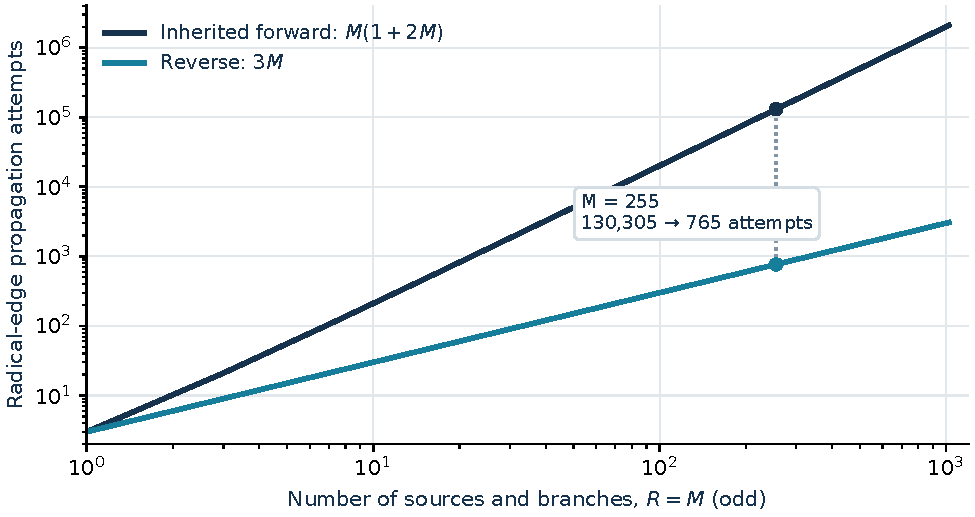
\includegraphics[width=\textwidth]{figures/directional_counts.pdf}
\caption{Exact radical-edge propagation counts for the shared-suffix
family with $R=M$ odd. The curves are the proved formulas, not fitted
timing data. At $M=255$, the ratio is $170\tfrac13$. Scalar setup and
the complete-stage bound are treated separately below.}
\label{fig:directional-counts}
\end{figure}

The counts are edge propagations or radical-edge visits.  They must not be
silently relabelled as cache misses, because many products in this family are
equal.  The implementation's typed identity shortcuts and coefficient caches
can avoid some actual algebra calls.  The repeated coefficient propagation
and accumulation in the forward graph remain, and the theorem states exactly
the operation count that it compares.

These two constructions are valid families of homogeneous algebraic
complexes.  They are not a theorem that arbitrary members arise at an
intermediate stage of scanning a knot diagram.  Establishing such a
realizability result, or finding comparably strong separation families of
actual residual knot diagrams, is a further research question.

\subsection{Compatibility with partial sparse cancellation}

Corridor transfer gives a complete exact alternative after a sparse
cancellation budget is exhausted.  Unlike the earlier support-only shortcut,
it also applies when survivors occupy adjacent degrees and their radical
differential is nonzero.  Because all maps are installed only after the
transfer finishes, the implementation can retain completed sparse pivots and
preserve the current state when a resource exception interrupts the proposed
replacement.  A failed budget or an unsuccessful support certificate is not
a topological verdict.

The operation counts identify two different opportunities: deleting data that
cannot reach a survivor, and avoiding repeated evaluation of a portion shared
by many sources or many targets.  They do not make the scalar survivor
profile smaller.  In particular, they do not resolve the possibility of very
large surviving multiplicities, nor the allocation cost of creating the next
crossing stage.  A general quasi-polynomial complexity theorem still requires
a uniform structural bound beyond the results proved here.

\subsection{Sparse scalar components and the cost of setting up transfer}
\label{sec:sparse-scalar-components}

The transfer counts in Section~\ref{sec:survivor-corridors} do not by themselves
bound the work of constructing $i,p,h$.  The inherited scalar implementation
groups all copies of one shifted matching into binary matrices and returns
columns as integer masks on the complete list of object slots.  A complex
with thousands of disconnected scalar identity pairs can therefore incur
large global masks even though its scalar contraction has only one nonzero
homotopy entry per pair.  That is a representation cost, not an algebraic
necessity.

We remove it by splitting the \emph{scalar} differential graph before doing
binary elimination.  Its vertices are the live original objects, and its
undirected edges are the nonzero entries of $d_0$.  These components are
direct summands of $(C,d_0)$, but usually not of $(C,d)$: radical entries are
deliberately excluded from this graph and may connect different components.
Every scalar component has one matching and one quantum shift, although it
can occupy several homological degrees.

For a singleton $a$, use the contraction with one survivor represented by
$a$, with its inclusion and projection both the identity and its homotopy
zero.  For a component consisting of the single scalar arrow
$a\to b=1$, use no survivor and put $h(b)=a$.  Every larger component is
remapped to its own local object indices, retaining the original relative
order, and processed by the inherited binary contraction.  Its output is
then converted to sorted tuples of nonzero original indices.  Columns of
$i,p,h$ are stored as these sparse tuples, rather than integers whose bit
positions range over all original objects.

\begin{theorem}[Scalar component contraction]
\label{thm:scalar-component-contraction}
The direct sum of the preceding local contractions is a typed special
contraction of $(C,d_0)$.  It preserves matching, quantum shift, and all
identities of Lemma~\ref{lem:corridor-binary}.  Suppose the scalar components
have sizes $\nu_1,\ldots,\nu_r$, and let $\mathcal B$ index those requiring
nontrivial local binary elimination.  The scalar construction admits the
conservative bound
\begin{equation}\label{eq:scalar-component-cost}
 \widetilde O\!\left(N+E+\sum_{j\in\mathcal B}\nu_j^3\right)
\end{equation}
in elementary bit operations, together with
\begin{equation}\label{eq:scalar-component-storage}
 O\!\left(N+\sum_{j\in\mathcal B}\nu_j^2\right)
\end{equation}
stored indices and local matrix entries.  Here $E$ is the number of all
stored differential entries, including radical entries, $N$ counts the original
slots, and the tilde suppresses logarithmic
factors for index manipulation, ordering, and the binary lengths of degree
and type labels.  Singleton and single-arrow components do not contribute a
cubic term.
\end{theorem}

\begin{proof}
The connected components of the scalar graph partition the objects into
subcomplexes, because every nonzero entry of $d_0$ has both endpoints in one
component.  All off-component matrix entries of $d_0$ vanish.  Taking direct
sums of the local identities $pi=1$, $d_0h+hd_0=1+ip$, and the side
conditions proves the corresponding global identities.  Local index changes
do not change matching or quantum shift, and the sparse tuple representation
changes no coefficient.

The scalar graph is constructed by inspecting every stored differential
entry, retaining scalar entries, and joining their endpoints.  The inspection
cost is $O(E)$, even if only a few entries are scalar.  Union by size with
path compression gives the usual
near-linear component calculation; a conservative logarithmic bound also
suffices here.  Each singleton or single arrow is processed in constant
local work and contributes a constant number of nonzero output indices.
For a component of size $\nu_j$, the inherited binary matrix operations have
a conservative cubic bit bound, with quadratic matrix storage.  Mapping
its output supports back to the original indices costs at most a quadratic
number of index operations.  The final ordering and index remapping incur
only the logarithmic factors displayed in~\eqref{eq:scalar-component-cost}.
Summing these costs proves the result.
\end{proof}

Merely taking direct sums would suffice for homotopy correctness, but it
could produce a different homology basis from the frozen reference.  For
entrywise validation of the new transfer we retain that reference basis
exactly.  The following ordering property makes this possible.

\begin{lemma}[Kernel anchors and compatibility of local bases]
\label{lem:scalar-kernel-anchors}
In the frozen scalar algorithm, process source columns in increasing
original object order and reduce them using the highest nonzero target
coordinate.  Every kernel candidate produced by a dependent column has
that column's source index as the largest index in its support.  Call this
index its anchor.  Computing separately on scalar components preserves all
selected kernel representatives, boundary bases, and boundary lifts.
\end{lemma}

\begin{proof}
When source column $a$ is processed, its tracked preimage begins with the
unit vector $e_a$.  Every pivot column available to reduce it was processed
earlier.  Its tracked preimage is supported on those earlier source indices.
Thus reductions can change only coordinates below $a$, and the coordinate
at $a$ stays one.  If the reduced image is zero, the resulting kernel
candidate has largest support index $a$.  Different dependent columns
therefore have different anchors.

For a scalar graph component, every column and tracked preimage is supported
within that component, and its image is supported within the same component
in the next degree.  Pivots from a different component have different target
support and cannot be used in its elimination.  A local remapping that
preserves the original order therefore encounters exactly the same relevant
pivots, in the same order, and constructs exactly the same images, lifts,
and kernel candidates.  Interleaving operations from different components
has no effect on these results.

The later selection of homology representatives starts with the boundary
basis and tests the kernel candidates in source order.  Boundary supports
from other components cannot affect independence in the given component.
The same candidates are consequently selected in both computations.  Finally,
the $B,H,L$ basis inversion is block diagonal with respect to these scalar
components, up to its explicit row and column ordering, so its local inverse
coefficients are also unchanged.
\end{proof}

\begin{corollary}[Exact reproduction of the frozen scalar basis]
\label{cor:scalar-exact-basis}
Merge the local survivor representatives in the order
\begin{equation}\label{eq:scalar-survivor-order}
 (\text{matching},q,h,\text{anchor})
\end{equation}
and remap the survivor indices in $p$ accordingly.  Then the sparse maps
$i,p,h$, converted to ordinary binary columns if desired, are entrywise
identical to the frozen reference maps.
\end{corollary}
\begin{proof}
The reference processes its scalar groups in order $(\text{matching},q,h)$.
Within each group it selects homology representatives in increasing order
of their dependent source columns.  By Lemma~\ref{lem:scalar-kernel-anchors},
that is precisely anchor order and the selected vectors are unchanged by
componentwise computation.  The inclusion columns therefore agree in both
their coefficients and their global order.  The local basis inversions
agree as well; applying the same survivor permutation gives the identical
projection, while the homotopy is independent of survivor numbering.
\end{proof}

The implementation avoids sorting a large list of survivors that already
have the same group key.  It places each representative at its original
anchor index, scans those slots once in increasing order, and appends the
representatives to their $(\text{matching},q,h)$ groups.  It then sorts only
the group keys.  Distinct anchors make the placement unambiguous.  This
also avoids constructing global integer bit masks during the merge.

\subsection{A complete sparse reduction bound for the separation family}
\label{sec:complete-sparse-separation}

The sparse scalar representation can be combined with a less expensive
direction policy.  Instead of constructing a separate packed reachability
label for every endpoint, one first computes two Boolean predicates:
reachable from some input, and able to reach some output.  These suffice to
prune to the corridor.  For a weak component with $a_j$ input ports and $b_j$
output ports, choose forward if $a_j\le b_j$ and reverse otherwise.  The
coarse bound~\eqref{eq:corridor-coarse-propagations} still holds; the fine
endpoint-mask bound is not being computed by this policy.

On general inputs, the port-count policy can make a worse choice than the
fine structural policy because different ports can reach very different
numbers of edges.  Its benefit is that graph setup uses only constant-size
Boolean labels.  Both policies compute the same exact differential and are
available separately so their setup and evaluation costs can be compared.

\begin{theorem}[Complete stage separation at fixed algebra size]
\label{thm:complete-sparse-separation}
Consider the shared-suffix family of
Theorem~\ref{thm:corridor-separation}, with $M$ odd.  Use sparse scalar
components, Boolean corridor pruning, and the port-count direction policy.
The complete reduction of its explicit two-term complex requires
\begin{equation}\label{eq:complete-sparse-family-cost}
 O((R+M)\log(R+M+2))
\end{equation}
word operations and $O(R+M)$ words of working storage, on a word RAM with
words large enough for its object indices.  The old forward evaluation
alone requires $\Omega(RM)$ coefficient-edge propagations.  For $R=M$ odd,
this yields a near-linear versus quadratic separation for the complete
reduction of this algebraic family, without omitting scalar setup.
\end{theorem}

\begin{proof}
The original complex has $N=R+2M+3$ objects, $M+1$ scalar identity edges,
and $R+2M$ radical edges.  Its scalar graph consists of $R+1$ survivor
singletons and $M+1$ single-arrow components.  The direct sparse construction
therefore uses only $R+1$ inclusion entries, $R+1$ projection entries, and
$M+1$ homotopy entries.  There is no nontrivial local binary problem.

The transfer graph has $2R+2M+4$ vertices and $2R+3M+2$ edges.  It is built
in linear work from these sparse supports.  Topological sorting contributes
at most the logarithmic factor in~\eqref{eq:complete-sparse-family-cost};
Boolean reachability and pruning are linear after the order is available;
component finding can be charged at most another linear-logarithmic term,
which is absorbed by the displayed bound. There is a single corridor with $R$ inputs and one
output.  The port policy chooses reverse for $R>1$; when $R=1$ either
direction has the same count.  Reverse evaluation uses $R+2M$ radical-edge
visits and $3M+2R+2$ total propagations, by
Theorem~\ref{thm:corridor-separation}.  It visits each graph vertex once for
the one output root.  All coefficients lie in the fixed eight-dimensional
algebra $\mathbb F_2[x,y,z]/(x^2,y^2,z^2)$, so their operations have constant
word cost.  The input, graph, sparse contraction, working coefficients, and
the $R$ output entries all occupy $O(R+M)$ words.

The inherited forward algorithm performs $R(1+2M)$ radical-edge visits on
this same input.  Even a perfect cache for repeated algebra products does
not remove its repeated propagation and accumulation along those edges.
This gives the stated lower bound and, with $R=M$, the separation.
\end{proof}

This strengthened result concerns the complete reduction of an already
explicit algebraic stage.  It still does not establish the realizability of
this family as knot-scan prefixes, beat the existing minimum-fill Gaussian
algorithm on every such input, or bound the size of every stage produced by
an arbitrary knot diagram.  Those are distinct questions.  Its contribution
is to remove a concrete representation obstruction that would otherwise
invalidate an end-to-end stage claim based only on the transfer counts.

\section{Complete cost accounting and the quasi-polynomial target}
\label{sec:accounting}

\subsection{A stage bound with every representation cost visible}

Fix one allocated partial complex. Let $N$ be its number of allocated
object slots, including slots made dead by previous cancellations,
$E_0$ the number of scalar differential entries, and $E_\delta$ the
number of radical entries between live objects. Put
$E_{\rm in}=E_0+E_\delta$. Let $s_1,\ldots,s_t$ be the sizes of the
weak components of the scalar graph. Write $M_{\rm sc}$ for the total
number of nonzero scalar entries retained in the sparse inclusion,
projection, and homotopy matrices. Object indices have
$O(\log(N+2))$ bits; a bound using only the live count would not
justify this assertion when many earlier slots are dead. Frontier
labels, matching identifiers, and the stored shifts contribute their
own input bit lengths.

For bit accounting, dictionary operations may be implemented by
deterministic ordered maps, with comparisons charged for their key
lengths. The resulting bounds describe the underlying algorithm;
the supplied Python implementation uses hash tables, whose timings
are reported separately. Even a conservative polynomial bound for
dictionary overhead leaves the conditional quasi-polynomial
conclusion below unchanged. We do not treat operations on arbitrarily
long Python integers as constant-time operations.

The componentwise scalar construction uses local binary matrices.
Classical elimination in a component of size $s$ has an
$O(s^3)$ binary-operation bound. The separately handled singleton and
one-edge components need constant local work each. Consequently a
conservative setup bound is
\begin{equation}
 A_{\rm sc}=
 \operatorname{poly}(\log(N+2)+\ell)\left(
 N+E_{\rm in}+M_{\rm sc}+\sum_{j:\,s_j>2}s_j^3\right),
 \label{eq:scalar-local-cost}
\end{equation}
where $\ell$ bounds the bit lengths of the non-index labels used by the
implementation. The $E_{\rm in}$ term is necessary: the construction
examines every differential entry to discover which ones are scalar.
Only a separately supplied scalar-edge index would permit charging
$E_0$ alone for that discovery. The displayed factor allows sorting
and integer-index operations; it is not intended as a
tight bit-level implementation model. The global predecessor can
instead pay cubic work in a whole matching/shift block even when that
block is disconnected, and stores global packed bit columns.

Across all adjacent homological degrees, the transfer graphs have
\[
 V=O(N+\mu),\qquad E=O(E_\delta+M_{\rm sc}),
\]
where $\mu\leq N$ is the number of scalar survivors. Each original
object appears in at most two adjacent-degree graphs, and each
relevant scalar matrix entry appears a bounded number of times. This
counts the graph representation, not only the retained corridors.

For a retained weak component $G_j$, let $V_j,E_j$ be its numbers of
vertices and edges, and let $a_j,b_j$ be its input and output counts.
The inexpensive endpoint policy chooses
\[
 r_j=\min(a_j,b_j)
\]
and evaluates from the corresponding side. It uses Boolean
reachability flags, not one packed endpoint set per vertex. Let
$\Lambda=\operatorname{poly}(\log(N+2)+\ell)$ absorb index,
dictionary, and ordering overhead. If $C(k,\ell)$ bounds the
arithmetic bit cost of a coefficient addition or typed composition
at a frontier of $2k$ endpoints, a full conservative stage bound is
\begin{equation}
 \begin{aligned}
 T_{\rm stage}\ &\leq A_{\rm sc}+A_{\rm graph}
   +\Lambda\sum_j V_jr_j\\
 &\quad+\Lambda(1+C(k,\ell))\sum_j E_jr_j.
 \end{aligned}
 \label{eq:full-stage}
\end{equation}
Here $A_{\rm graph}$ includes reading all initial graph edges,
topological ordering, pruning, and connected-component construction.
For the Boolean endpoint policy they admit a bound polynomial in
the index and label lengths times $N+V+E$. Initializing the $\mu$
output rows is included; writing a nonzero output coefficient is
charged to its terminal propagation, up to a constant factor. The
$V_jr_j$ term is required because the implementation visits the
component's ordered vertex list once for each chosen endpoint, even
when a particular coefficient is zero.

The finer reach-set policy replaces the edge sum by
$\sum_j\min(F_j,B_j)$ with unit edge weights, as proved in the
preceding section. In the vertex term, $r_j$ must then be the
number of endpoints on the \emph{actually chosen side}: a smaller
reach-set bound need not choose the side with fewer endpoints.
It must additionally pay for the packed reachability sets, with
a conservative $O((V+E)\mu)$ bit-operation term, apart from index
and label overhead. In particular, an OR or a population count on
a $\mu$-bit endpoint set is not one bit operation. This policy's
tighter propagation count can be outweighed by its larger setup cost.

With the existing dense coefficient engine, one may take
$C(k,\ell)=\operatorname{poly}(k,\ell)2^{O(k)}$. A claim about a
particular software configuration must use the coefficient engine
actually selected; the sparse default may inspect more monomial
pairs. Equation~\eqref{eq:full-stage} remains valid with the
corresponding conservative composition bound.

\subsection{Why the sparse refinement matters}

Even a column containing a single bit at global position $j$ takes
$j+1$ bits when stored as the integer $2^j$. Thus $R$ unrelated
singleton inclusions stored at positions $0,\ldots,R-1$ use
\[
 \sum_{j=0}^{R-1}(j+1)=R(R+1)/2
\]
bits of packed integer payload. Their sparse index lists use
$O(R\log(N+2))$ bits. This is a representation effect, independent
of the mathematical sparsity of the contraction.

On the shared-suffix family proved above, every scalar component is
a singleton or one identity pair. The componentwise scalar setup has
linear nonzero count, and the Boolean endpoint policy avoids the
quadratic packed reach-set volume. Reverse transfer then has
$R+2M$ radical-edge propagations, whereas the inherited forward
transfer has $R(1+2M)$. Reading the input and writing the $R$ output
coefficients are still required.

More precisely, the complete-stage separation theorem applies to
the explicitly constructed family with $M$ odd, the fixed
eight-dimensional dot algebra on one three-arc matching, sparse
scalar components, Boolean corridor flags, and the automatic
endpoint-count policy. There are $R+2M+3$ objects and $O(R+M)$
input entries, scalar supports, graph vertices, and graph edges.
For $R>1$ its one output endpoint makes the policy choose reverse
evaluation, which visits the graph once; for $R=1$ either direction
has the same bound. With generic ordering, the complete reduction uses
$O((R+M)\log(R+M+2))$ word operations and $O(R+M)$ words.
Words here contain the object indices and labels of this family;
their size is $O(\log(R+M+2))$ bits. A conservative bit implementation
therefore has a near-linear bound with additional logarithmic
factors, rather than a claimed linear bit cost.

For $R=M$ odd, inherited forward propagation alone performs
$\Omega(M^2)$ operations. The fixed coefficient algebra is essential
to this comparison: coefficient sizes are constant in this family.
This establishes the stated stage separation while including
scalar setup, and does not imply a linear running time for arbitrary
knot scans or superiority over ordinary minimum-fill cancellation.

\subsection{What still prevents a general scanner bound}

The current scanner explicitly allocates its objects before reducing
them. Neither the number of matching types nor a small boundary
alone bounds their multiplicities. The new reducer cannot avoid
reading an explicitly supplied complex of size $N$, and its minimal
output may itself contain exponentially many objects. Choosing better
scalar bases may reduce fill and corridor sizes; it does not change
the graded scalar homology dimensions of a fixed prefix.

For example, consider diagrams with normalized edge labels, charging
normalization of a longer external encoding at its actual input
bit cost. Suppose an order is supplied or constructed within the
target quasi-polynomial budget, and an execution satisfies
$N_i\leq\exp(O(\log^2(n+2)))$ and
$k_i=O(\log^2(n+2))$ at every stage, with label and shift bit lengths
polynomial in $n$. Here $N_i$ bounds each allocated stage before
reduction, including retained dead slots. Then $E_{{\rm in},i}$ and
$M_{{\rm sc},i}$ are polynomial in $N_i$, as are all graph and
endpoint counts. The setup bounds, coefficient envelope, and the
ordinary polynomial-cost crossing-extension operations on these
explicit tables make the complete $n$-stage scan quasi-polynomial.
This is sufficient accounting under explicit execution and
encoding hypotheses. There is no proof here that arbitrary diagrams
admit orders satisfying those hypotheses. The remaining research task
is to prove a structural bound or devise a representation that avoids
the explicit-object lower bound.

The same caution applies to the corridor support. Its form depends
on the chosen scalar contraction, so it is not a knot invariant and
is not canonical under arbitrary scalar basis changes. A dense basis
change can enlarge inclusion, projection, and homotopy supports while
leaving the homotopy type unchanged.

\subsection{What the covering theorem supplies to a hierarchy}

Suppose a compressed cutting step exposes a parallelity-bundle base
as a valid dihedral cover of a smaller bordered surface. The
three-family theorem then supplies the base topology, the orientation
interval-bundle type, and marked boundary lookup in time polynomial
in the presentation length and the bit length of its sheet count.
This removes a possible dependence on the expanded number of sheets
for that promised input class.

The general compressed cutting theorem of Lackenby is broader and is
already stated with logarithmic dependence on normal-surface weight
\cite[Theorem 14.4]{Lackenby2026}. Our contribution is an explicit,
small, checked kernel and classification for a restricted arithmetic
presentation. It should not be described as a new proof of the
general theorem. External attaching maps remain indispensable: two
components with the same intrinsic topology can attach differently
to the nonparallel part of a three-manifold.

\subsection{Hierarchy depth, restarts, and conditional arithmetic}

Lackenby's Section 9 yields the iteration bound
\begin{equation}
 L(g+1)^L,
 \label{eq:lackenby-iterations}
\end{equation}
where $L$ bounds hierarchy length and $g$ bounds decomposing-surface
pattern complexity \cite[Proposition 9.1]{Lackenby2026}. The integer
potential responsible for the bound is a base-$(g+1)$ encoding of the
successive complexities. A strict decrease proves termination; the
size of the integer still determines the worst possible number of
restarts. Section 10 obtains a linear bound on $L$ in the initial
handle complexity after additional parallelity-bundle operations.
Linear depth alone does not make \eqref{eq:lackenby-iterations}
quasi-polynomial.

The polynomial simplification statement of Proposition 14.2 assumes
an irreducible manifold with essential boundary pattern. Its use
inside a recognizer must respect that hypothesis. A short certificate
for an essential hierarchy also does not give a deterministic search
procedure with the same cost.

A prospective complete algorithm would be quasi-polynomial if it
visited at most $\exp(O(\log^2 n))$ compressed states, each state had
polynomial or quasi-polynomial bit size, and each required transition
had a correspondingly bounded verified implementation. The two
kernels reduce specific transition or representation costs. They do
not prove the state-count hypothesis. This is the exact remaining
gap between the delivered results and the user's global objective.

\section{Verification and measured performance}
\label{sec:experiments}

The algebraic separation theorems and the observed performance lead to
different conclusions. Corridor transfer removes provably unnecessary
work from the inherited forward transfer, and its sparse scalar variant
removes a quadratic representation cost on the explicit separation
family. On the ordinary diagram scans measured here, however, the
production sparse reducer remains substantially faster. This section
reports both conclusions, with the controls needed to interpret them.

\subsection{What the verification checks}

The algebraic tests compare several levels of information. Before and
after ordinary cancellation, the full
\((\text{matching},h,q)\) survivor profile is checked against scalar
homology, together with quantum homogeneity and \(d^2=0\). On allocated
prefixes, the new transfer is compared entrywise with the frozen
one-sided implementation in the same scalar-contraction basis, in
forward, reverse, and automatic modes, with pruning both enabled and
disabled. Selected cases also check all eight full contraction
identities in the cobordism algebra. These checks include parity
cancellation: a nonempty corridor can have zero path sum over \(\F\).
Boolean reachability is never interpreted as a nonzero coefficient.

An independent set-valued coefficient engine with a different pivot
order checks the final homological-degree ranks on seeded diagram
families. Sparse scalar-component tests convert every tuple column
back to a binary mask and compare inclusion, projection, and homotopy
entrywise with the frozen scalar construction. Further tests exercise
dead object slots, partially completed ordinary cancellation, tail
contraction, the component coefficient engine, and resource failure.
The complete scanner suite passes \(268\) tests: \(245\) baseline
tests, eight graded-support tests, ten corridor tests, and five
scalar-component tests. Its recorded run took \(30.764\) seconds;
the package retains the log and final verification manifest.
These finite checks support the implementation; they do not replace
the general proofs.

The geometric kernel has a separate expanded-sheet oracle. It
constructs the lifted graph, finds its connected components by graph
search, propagates orientation parity along lifted edges, and
enumerates boundary permutations. The oracle does not reuse the
classifier's gcd calculation, boundary-word evaluator, or canonical
schema constructor. The supplied campaign comprises \(13{,}846\)
topology comparisons, including exhaustive low-rank assignments and
\(2{,}000\) seeded larger schemas. Additional checks cover fibre
relabeling, explicit generic equivariance, exhaustive bijections for
small exceptional covers, malformed inputs, and small moduli.

The large-integer test uses the reflection action over a M\"obius
band with \(W=2^{10000}\) sheets. It returns three family records,
two cover-isomorphism types, and \(2^{9999}+1\) connected components
without expanding them. This verifies the intended compressed output
contract; it is not a benchmark of normal-surface extraction or
unknot recognition.

\subsection{Timing protocol and baselines}
\label{sec:timing-protocol}

The principal measurements are recorded in
\path{fast/results/corridor_benchmark_20261008.json}, generated by
\path{fast/benchmark_corridor.py}. The software environment recorded
in the file is Python \(3.12.14\) on Linux \(6.18.44\), x86-64, with
glibc \(2.39\). Each case has seven paired rounds, with the order of
the arms shuffled by a fixed seed. Every implementation is warmed
before measurement. A warm pilot selects a fixed repetition count
for each arm, targeting a \(20\)-millisecond batch, capped at
\(32\) repetitions. The two identical sparse-control arms use the
same repetition count.

For actual diagrams, a fresh scanner is constructed on every
repetition and the complete raw scan is timed. All arms receive the
same precomputed crossing order and the same scanner-level
shape-cache setting. Diagram construction, common order selection,
and explicit verification are excluded. No braid, Seifert,
Alexander, Jones, Reidemeister, or factorization front end is being
credited with a speedup in this experiment. For synthetic complexes,
construction is excluded and the complete reduction of a fresh
allocated complex is timed. Scalar contraction, graph construction,
pruning, direction selection, and output installation are included.

Before each measured batch the garbage collector is collected; it
remains enabled during timing. Every scanner has a cooperative
\(30\)-second deadline. Other team agents paused CPU-intensive work
during the final coordinated runs. Earlier exploratory timing files
are retained as provenance but are not the primary dataset.

The nine arms are the production sparse scanner, an identical sparse
control, quantum bookkeeping with the ordinary reducer, the frozen
one-sided transfer, forward corridor evaluation without pruning,
forward evaluation with pruning, reverse evaluation with pruning,
automatic direction selection with pruning, and adaptive corridor
reduction. The automatic full-transfer arm uses the original global
scalar construction and packed endpoint reach sets. The later
sparse-component/Boolean variant is measured separately.

All times in the tables are medians of per-run batch times. Ratios
are computed within each paired round and then summarized by their
median; consequently a reported ratio need not equal the ratio of
the two displayed median times. An \(A/A\) ratio compares the two
identical sparse implementations. Across the principal cases these
ratios range from \(0.755\) to \(1.399\), despite the controls.
Absolute timings and small differences therefore deserve
considerable caution. We report large deterministic count
reductions separately from elapsed-time ratios, and do not promote
small apparent gains into general performance claims.

\subsection{A negative result for the stronger support certificate}

The full grading allows the zero-differential certificate of
Proposition~\ref{prop:corridor-typed} even when consecutive
homological degrees survive. The audit
\path{fast/audit_graded_support.py} evaluates this certificate and
the earlier degree-gap certificate on exactly the same unreduced
prefixes, then checks the predicted profile against ordinary
cancellation.

Its \(72\) actual diagrams consist of twelve fixed fixtures or
families and sixty seeded random braid closures. Across \(639\)
stages, both certificates succeed on exactly \(196\) stages; the
full graded certificate supplies \emph{zero additional successes}.
The ordinary reductions perform \(3{,}470\) Schur-update pairs.
The complete records are in
\path{fast/results/graded_support_20261008.json}.

This does not weaken the support theorem. It shows that a strictly
stronger sufficient condition need not improve the supplied
execution family. It also explains why the implementation effort
proceeds to complete transfer, which retains nonzero radical
differentials, instead of assuming that a better all-zero test will
usually suffice.

\subsection{Actual raw diagram scans}

Table~\ref{tab:actual-corridor} gives the main actual-diagram result.
The first case is the closure of the \(201\)-letter positive
two-braid. The next two are the closures of
\((\sigma_1\sigma_2)^{10}\) and
\((\sigma_1\sigma_2^{-1})^4\). The remaining cases use the supplied
Morton, Conway, and hard eight-crossing fixtures. The exact PD codes
and crossing orders are recorded in the JSON.

\begin{table}[htbp]
\centering
\small
\setlength{\tabcolsep}{4pt}
\begin{tabular}{@{}lrrrrrr@{}}
\toprule
Case & Sparse ms & Full ms & Adaptive ms &
Sparse/full & Sparse/adapt. & \(A/A\)\\
\midrule
Two-braid, \(201\) & 124.044 & 1324.193 & 192.852 & 0.094 & 0.679 & 0.913\\
Torus \(3,10\) & 8.936 & 29.650 & 9.692 & 0.311 & 0.954 & 1.268\\
Alternating three-braid & 5.059 & 14.435 & 4.705 & 0.367 & 1.141 & 1.009\\
Morton & 2.075 & 4.801 & 2.351 & 0.412 & 1.026 & 0.947\\
Conway & 5.828 & 17.704 & 6.937 & 0.319 & 0.864 & 0.878\\
Hard unknot, \(8\) & 1.195 & 2.796 & 1.335 & 0.475 & 0.934 & 0.938\\
\bottomrule
\end{tabular}
\caption{Complete raw scans. \emph{Full} means automatic pruned corridor
transfer at every reduction stage. A ratio greater than one would
favor the corresponding corridor arm.}
\label{tab:actual-corridor}
\end{table}

Full corridor reduction is approximately \(2.1\)--\(10.7\) times
slower than the production sparse class on these cases. It can
remove a substantial fraction of the graph while still losing
overall, because binary contraction and graph setup must be paid
at every stage. This is a measured total-cost failure, not a
failure of coefficient correctness: all final ranks by homological
degree agree.

The adaptive arm performs no corridor switches on any of these six
cases. Its sparse-work allowance is never exceeded. Thus the modest
variations in its timing cannot be attributed to successful use of
corridor transfer. The data support retaining ordinary sparse
cancellation as the default; they supply no reliable general
actual-diagram speedup from either new strategy.

\subsection{Homogeneous algebraic families with nonzero transfer}

The synthetic tests are valid two-term complexes in the same
graded category. Since they occupy only homological degrees zero
and one, their square-zero condition is automatic; quantum
homogeneity is checked explicitly. They are not asserted to occur
as prefixes of any supplied classical knot diagram.

The seeded dense family uses one matching with three arcs.
Surviving sources have quantum shift \(0\), surviving targets have
shift \(6\), and two scalar contractible layers have shifts \(2\)
and \(4\). Radical matrices between successive layers are
multiplied by \(x,y,z\), respectively. Each scalar layer has
sixteen contractible pairs. Source-heavy and target-heavy cases
use multiplicities \(64:1\) and \(1:64\); the balanced case uses
\(16:16\). The dense dead-branch case adds sixty-four contractible
pairs at each intermediate shift on branches that cannot reach a
surviving target.

The strict shared-suffix cases use the sparse family of
Theorem~\ref{thm:corridor-separation}, with \(R=M\) odd. The
dead-leaf case uses Proposition~\ref{prop:corridor-dead} with
\(255\) irrelevant contractible leaves. Every displayed strict
case has nonzero transferred differential. Thus the reductions
cannot be explained by an all-zero shortcut.

\begin{table}[htbp]
\centering
\small
\setlength{\tabcolsep}{5pt}
\begin{tabular}{@{}lrrrr@{}}
\toprule
Family & Prior attempts & Corridor attempts &
Prior/corridor & Sparse/corridor\\
\midrule
Dense source-heavy & 3,940 & 307 & 3.631 & 0.506\\
Dense target-heavy & 317 & 317 & 0.365 & 0.243\\
Dense balanced & 2,142 & 2,142 & 1.070 & 0.397\\
Dense dead branches & 72,204 & 342 & 9.690 & 1.346\\
Shared suffix, \(15\) & 465 & 45 & 1.975 & 0.157\\
Shared suffix, \(63\) & 8,001 & 189 & 7.091 & 0.105\\
Shared suffix, \(255\) & 130,305 & 765 & 28.409 & 0.098\\
Dead leaves, \(255\) & 256 & 1 & 0.498 & 0.120\\
\bottomrule
\end{tabular}
\caption{Radical-edge product attempts and paired total-reduction
timing ratios. The prior is the frozen one-sided transfer; the
corridor arm uses automatic direction and pruning. Synthetic
construction is excluded, but scalar and graph setup are included.}
\label{tab:kernel-corridor}
\end{table}

The operation counts in Table~\ref{tab:kernel-corridor} compare the
same event: propagation across a radical edge, requiring a typed
coefficient product. They do not compare the predecessor's raw
algebra-call counter directly with the new implementation's
composition counter. The latter excludes typed identity shortcuts
and may use cached products. Scalar propagations are distinguished
from radical attempts; vertex-loop and setup costs remain included
in the elapsed times.

At \(R=M=255\), the exact formulas give
\[
 R(1+2M)=130{,}305,\qquad R+2M=765.
\]
The radical-edge reduction factor is \(170\frac13\), while the
measured total reduction is about \(28.4\) times faster than the
inherited forward sweep. Ordinary Markowitz cancellation is still
about ten times faster than the full corridor method on this
family. Its pivot order already exploits the shared structure
effectively. The theorem proves an unbounded improvement over a
specified inherited transfer, not superiority over every exact
reduction strategy.

The dead-leaf example makes the setup issue especially clear:
radical attempts drop from \(256\) to \(1\), yet total reduction
becomes slower than the prior. Conversely, the dense dead-branch
case has a modest apparent \(1.35\)-fold gain over sparse reduction.
Given the identical-control drift, we do not treat that single
ratio as dependable practical superiority.

All full-transfer arms produce exactly the same minimal
differential in the frozen scalar basis; the benchmark records its
SHA-256. Ordinary and adaptive sparse reductions may select a
different homogeneous basis. They are checked independently by
survivor multiplicities and by the binary rank of the coefficient
matrix of the single possible output monomial, \(xyz\) or \(x\).
For this planted family those quantities are preserved by the
allowed homogeneous changes of basis.

\subsection{The sparse scalar refinement: a separate negative timing test}

After the principal experiment was frozen, a targeted follow-up combined
sparse scalar components, Boolean reachability, and direction selection
by port count. It compared this variant with the frozen corridor's
forward and automatic modes, the port-count policy with
global scalar setup, and two identical production sparse arms.
This keeps the effect of the new setup representation separate from
the original direction/pruning result. Its data are in
\path{fast/results/compressed_corridor_20261008.json}.

\begin{table}[htbp]
\centering
\small
\setlength{\tabcolsep}{5pt}
\begin{tabular}{@{}lrrrrr@{}}
\toprule
Case & Frozen auto ms & New sparse ms &
Auto/new & Production/new & \(A/A\)\\
\midrule
Two-braid, \(201\) & 1269.243 & 1448.700 & 0.803 & 0.091 & 1.087\\
Conway & 20.762 & 26.421 & 0.804 & 0.292 & 1.110\\
Hard unknot, \(8\) & 2.746 & 2.866 & 0.934 & 0.441 & 0.795\\
Shared suffix, \(15\) & 0.562 & 0.423 & 1.250 & 0.174 & 1.191\\
Shared suffix, \(63\) & 1.672 & 1.422 & 1.202 & 0.132 & 1.056\\
Shared suffix, \(255\) & 7.847 & 8.178 & 0.871 & 0.101 & 1.011\\
Dead leaves, \(255\) & 2.663 & 2.392 & 1.113 & 0.154 & 0.997\\
\bottomrule
\end{tabular}
\caption{The targeted sparse-setup follow-up. \emph{New sparse} means
sparse scalar components, Boolean pruning, and port-count direction
selection, not the production sparse cancellation algorithm.}
\label{tab:compressed-setup}
\end{table}

There is no stable practical timing gain at these tested sizes. The
refinement loses on all three actual examples and on the largest
shared-suffix instance; the small apparent gains elsewhere are
comparable to control variation. Its justification is the exact
representation and complete-stage bound, not a claim that Python
tuples and extra component bookkeeping are always faster.

\subsection{Exact representation counts}

The additional audit
\path{fast/audit_scalar_representation.py} compares all scalar
matrices entrywise and records representation sizes in
\path{fast/results/scalar_representation_20261008.json}. In the
shared-suffix constructor's fixed object order, the sum of the
integer bit lengths of all inherited \(i,p,h\) columns is
\[
 R^2+4R+5+MR+\frac{M^2+9M}{2}.
\]
At \(R=M\), this is \((5M^2+17M+10)/2\). The sparse representation
has exactly \(2R+M+3\) nonzero indices, each requiring only the
binary length of an object or survivor index.

For completeness, the constructor orders the sources first, then
\(L_0,B_0\), then all \(L_i\), then all \(B_i\), and finally
\(t\). The separate sums of bit lengths are
\[
\begin{aligned}
 |i|_{\rm bits}&=R(R+1)/2+R+2M+3,\\
 |p|_{\rm bits}&=R(R+1)/2+R+1,\\
 |h|_{\rm bits}&=R+1+\sum_{i=1}^{M}(R+i+2).
\end{aligned}
\]
Adding proves the displayed polynomial. There are respectively
\(R+1\), \(R+1\), and \(M+1\) nonzero scalar entries, proving the
sparse count. Other object orderings can change the packed-bit
polynomial, while the sparse nonzero count is unchanged for this
direct contraction.

\begin{center}
\small
\begin{tabular}{@{}rrr@{}}
\toprule
\(R=M\) & Packed integer bit length & Sparse indices\\
\midrule
1 & 16 & 6\\
3 & 53 & 12\\
15 & 695 & 48\\
63 & 10,463 & 192\\
255 & 164,735 & 768\\
\bottomrule
\end{tabular}
\end{center}

For \(M=255\), there are \(768\) original objects and \(512\)
scalar components: \(256\) singletons and \(256\) identity pairs.
No component requires nontrivial binary elimination. This is the
situation in which sparse setup makes the complete-stage separation
possible. The table measures integer payload length and support
counts, not actual Python heap allocation; object and tuple
overheads can dominate at small sizes.

The experiments therefore leave a clear deployment decision.
Preserve the production sparse default, retain the new kernels as
exact opt-in research capabilities, and use the supplied counters
to identify inputs where setup is amortized. A universal
quasi-polynomial bound still requires the structural hypotheses
discussed in Section~\ref{sec:accounting}.

\section{Software integration and exact interfaces}
\label{sec:integration}

The supplied scanner changes are optional. The public default remains
\code{reduction="standard"}, which selects the existing sparse
minimum-fill cancellation. Earlier structural tests and recognition
decisions retain their existing order. Selecting a new reducer changes
the chain-complex calculation only if execution reaches that stage.
The dihedral-cover classifier is a separate topology kernel; it is not
silently substituted for a normal-surface or knot-recognition routine.

\subsection{Scanner modules and their responsibilities}

The new scanner code is organized by mathematical responsibility.
The following filenames are relative to \path{fast/fastunknot/}.

\begin{center}
\small
\begin{tabularx}{\textwidth}{@{}p{0.31\textwidth}X@{}}
\toprule
Module & Contract\\
\midrule
\code{graded.py} &
Retains raw quantum shifts, checks homogeneous degrees, predicts the
full scalar survivor profile, and supplies support-only reference
reducers.\\
\code{binary_contraction.py} &
Preserves the inherited scalar-contraction basis and its global
packed-column representation.\\
\code{scalar_components.py} &
Splits the scalar graph into components, handles isolated objects
and identity pairs directly, and returns sparse index columns in
the same survivor basis.\\
\code{corridor.py} &
Constructs the typed transfer graph, prunes irrelevant paths,
evaluates either direction, and installs the full minimal
differential through scanner-compatible classes.\\
\bottomrule
\end{tabularx}
\end{center}

The quantum array is aligned with the scanner's object slots.
Ordinary cancellation can leave dead slots, and the grading code
preserves that convention. Crossing expansion installs the new shifts
before dispatching to the chosen reducer. The shifts are the raw
scanning shifts of equation~\eqref{eq:corridor-q-recurrence}; no
diagram-wide orientation normalization is silently applied.

The direct kernel \code{corridor_transfer(scan)} requires a valid
homogeneous chain complex in the scanner category. It returns the
surviving matching, homological-degree, and quantum-shift arrays, the
full output differential, the scalar contraction, component details,
and work counters. The original object and differential arrays are
not replaced by this function, although coefficient caches can be
populated. \code{CorridorScan} performs the replacement after the
kernel completes.

\subsection{Public recognition and raw-homology options}

Two reduction names are added to \code{khovanov_rank},
\code{recognize}, and their corresponding command-line commands:
\begin{description}
\item[\code{corridor}]
Compute the full survivor differential by scalar contraction and
automatic bidirectional transfer through the retained corridors at
every reduction stage.
\item[\code{corridor-adaptive}]
Start with the existing sparse reducer and permit
\(\max(256,4N)\) candidate Schur-update pairs at the beginning of
the stage, where \(N\) is the current live object count. If the
allowance is exceeded, retain completed pivots and transfer the
partially reduced complex.
\end{description}

The allowance is a heuristic for when to pay for another
representation. It has no competitive-time guarantee. It also
differs from the older \code{adaptive} reducer: that method tries a
zero-differential survivor-profile certificate and resumes ordinary
cancellation when the certificate is inconclusive. The new adaptive
method can finish with a nonzero radical differential.

A raw-homology call bypasses the recognition front ends and therefore
provides a direct way to exercise the selected reducer:

\begin{lstlisting}[language=Python]
from fastunknot import Diagram, khovanov_rank

diagram = Diagram.from_braid(3, [1, -2] * 4)
result = khovanov_rank(
    diagram.pd,
    reduction="corridor-adaptive",
    max_objects=50000,
    seconds=30,
    check_d_squared=True,
)
print(result["rank"], result["by_degree"])
\end{lstlisting}

The returned public quantities retain their prior conventions:
\code{rank} is the unreduced \(\F\)-rank,
\code{reduced_rank} is half of it for a knot, and
\code{by_degree} uses the raw homological degrees.
The result records the nonstandard reduction name and its counters.
The direct graded scanner additionally exposes
\code{ranks_by_bidegree()}; its live-object counts are homology
dimensions only once the differential has been shown to vanish,
as on a closed minimal complex.

The corresponding command-line examples, run inside \path{fast/},
are:

\begin{lstlisting}
python -m fastunknot khovanov examples/conway.json \
  --reduction corridor --check-d2

python -m fastunknot recognize examples/conway.json \
  --reduction corridor-adaptive \
  --seconds 30 --max-objects 50000
\end{lstlisting}

The recognition command can finish in an earlier certified stage,
so a chosen reduction option does not imply that a scan occurred.
Inspect the returned method and scan evidence when measuring it.
The option \code{--no-reduction} retains its previous meaning:
it disables Reidemeister preprocessing. It is unrelated to the
\code{--reduction} chain-cancellation selector.

\subsection{Research controls for direction and scalar setup}

The public reduction names use
\code{mode="auto"}, \code{prune=True},
\code{direction_policy="reach"}, and
\code{scalar_engine="global"}. The sparse scalar variant is exposed
through the direct scanner/kernel API, allowing the additional setup
choices to remain independently measurable:

\begin{lstlisting}[language=Python]
from time import monotonic
from fastunknot.corridor import CorridorScan
from fastunknot.ordering import best_scan_order

scan = CorridorScan(
    mode="auto",
    prune=True,
    direction_policy="ports",
    scalar_engine="components",
    max_objects=50000,
    deadline=monotonic() + 30,
)
for index in best_scan_order(diagram.pd):
    scan.add_crossing(diagram.pd[index])
print(scan.total_rank())
\end{lstlisting}

This example continues with the validated nonempty diagram above.
For ordinary use, the public raw-homology API also handles its
established zero-crossing convention and other dispatch details.

The \code{mode} values are \code{forward}, \code{reverse}, and
\code{auto}. Disabling pruning supplies an ablation rather than a
different homotopy invariant. The \code{reach} policy constructs
packed endpoint sets and minimizes the finer structural propagation
bound separately in each weak component. The \code{ports} policy
uses Boolean reachability and compares the component's numbers of
input and output ports. It avoids endpoint-mask setup but can choose
a direction with a worse fine-grained bound. Neither policy is
described as an oracle for elapsed time.

The \code{global} scalar engine retains the frozen construction.
The \code{components} engine uses the sparse direct-sum construction
proved above. These controls can also be passed to
\code{AdaptiveCorridorScan}. There is no additional public
\code{corridor-compressed} reduction name in this release.

\subsection{Compatibility and resource semantics}

The supported combinations are explicit:

\begin{center}
\small
\begin{tabularx}{\textwidth}{@{}p{0.28\textwidth}X@{}}
\toprule
Option or interface & Corridor requirement or behavior\\
\midrule
Scanner backend &
The standard scanner backend; the shared, saturated, Euler, and
twist backends are outside this integration.\\
Pivot and algebra &
\code{pivot="minfill"}, \code{algebra="bits"}, and
\code{self_inverse=True} in the raw API.\\
Racing &
\code{race=1}; competing scan processes are not combined with these
reducers.\\
Coefficient composition &
The standard, component, and forced component-dense coefficient
engines remain selectable subject to their existing limits.\\
Tail contraction &
Permitted. The requested final crossings are added without
cancellation, then the closed scalar complex is finished by the
existing binary rank calculation.\\
Homological windows &
The public corridor recognition options require
\code{window_radius=None}. The separate window command retains
its existing reduction choices.\\
\bottomrule
\end{tabularx}
\end{center}

Incompatible raw-API combinations raise \code{ValueError}. The CLI
rejects incompatible backend, algebra, pivot, racing, sharing, twist,
and corridor/window combinations as option errors. These guards
prevent a requested reducer from being silently replaced by an
unsupported implementation.

The object ceiling is checked before crossing expansion allocates
the predicted number of objects. It is a ceiling on that count,
not a limit on total Python memory or on all auxiliary scalar
matrices. Time limits are cooperative: scalar setup, graph
construction, reachability, and propagation poll the ordinary
resource checks. They are not operating-system hard deadlines.

The transfer computes its replacement before installing new object
and map arrays. A resource failure during that calculation therefore
does not install an incomplete minimal differential. Adaptive
reduction retains any complete sparse pivots already performed.
This statement concerns the reducer; it does not assert that every
allocation or entire crossing-expansion operation is reversible.

The raw \code{khovanov_rank} API propagates \code{ScanLimit} and
\code{MemoryError}. The recognition pipeline catches both and
returns \code{UNKNOWN} with resource evidence. The raw CLI likewise
reports a resource failure rather than a knot verdict. Exhausting
an object or time allowance never means that a knot has been found,
and an empty set of usable shortcuts never means that a diagram is
an unknot.

\subsection{Counters and reproducible comparisons}

The \code{corridor_} counters expose original and retained graph
sizes, component counts, selected directions, structural forward
and reverse bounds, actual edge propagations, radical-edge
propagations, coefficient xors, and nontrivial compositions.
\code{corridor_switches}, when present, records adaptive transitions
from sparse cancellation. Stage histories retain the input and
survivor counts.

The structural-bound assertion checks that the counted
propagations do not exceed the chosen bound. That assertion does
not count all execution costs: the component's ordered vertices
must still be visited, and scalar/graph setup remains necessary.
The distinction is reflected in
equation~\eqref{eq:full-stage} and in the negative timings.

The package keeps both frozen predecessors, the measured source
hashes, full input descriptions and crossing orders, raw timing
batches, and exact matrix digests. The reproduction wrapper restores
the required frozen corridor in a temporary copy when replaying the
nine-arm experiment, so historical measurements can be reproduced
without overwriting the delivered implementation. The separate
compressed-setup experiment uses the frozen corridor as an explicit
baseline. The ordinary test suite and the two inexpensive support
audits can be run independently of the timing campaigns.

\subsection{The covering classifier is an explicit separate contract}

The geometric implementation is
\path{dihedral_covers/dihedral_cover.py}. Its input schema specifies
an orientable bordered surface by genus and boundary count, or a
nonorientable bordered surface by crosscap and boundary counts,
together with a positive sheet count and one affine permutation for
each canonical free generator. Shifts are reduced modulo the sheet
count. The canonical schema supplies the boundary words and
orientation character, so accepted data do not depend on checking
an omitted closed-surface relation.

\begin{lstlisting}
python dihedral_covers/dihedral_cover.py \
  dihedral_covers/examples/three_types.json
\end{lstlisting}

The Python entry points are \code{classify_cover},
\code{component_key}, and \code{boundary_lift_key}. The first returns
at most three component-family records, their multiplicities,
covering degrees, surface topology, complete boundary-degree
profiles, and cover-isomorphism type identifiers. Distinct
exceptional residue records can share a type identifier while
remaining separately queryable. The two marked-query functions
identify the component and lifted boundary circle containing a
specified fibre point without expanding the sheets.

The field \code{orientation_interval_bundle} describes the
canonical interval bundle with orientable total space. It does not
specify an arbitrary extra twisting character. Unknown fields,
incorrect generator counts, invalid signs, inappropriate surface
parameters, and booleans supplied in place of integers are rejected.

This schema certifies an abstract finite surface cover. Extracting
that schema from a normal surface, certifying an embedding in a
three-manifold, and retaining arbitrary external attaching maps
are separate tasks. No current scanner or recognizer dispatches to
this classifier merely because a large integer weight appears.
The integration point for a future compressed cutting backend must
supply the covering presentation and its attachment data
explicitly, as required in Section~\ref{sec:accounting}.

\section{Research agenda: precise next theorems and experiments}
\label{sec:research}

The next stage should prioritize questions that either remove an identified
asymptotic obstruction or determine whether the new kernels accelerate
actual difficult inputs. The following questions are deliberately stated
with success criteria. A negative answer can also be valuable: an explicit
obstruction prevents effort being spent on an insufficient invariant or
representation. These are proposed research problems, not claims that the
necessary bounds have been proved.

\subsection{Near-term algebra and implementation}

\begin{researchquestion}[Realization of directional separation]
Can a family of actual knot diagrams and legal scan prefixes realize the
shared-suffix transfer structure of Theorem~\ref{thm:corridor-separation},
up to uniformly bounded local modifications?
\end{researchquestion}

The algebraic construction has fixed matching width and a nonzero
three-dot output, so its separation is not an artifact of an invalid
differential or zero answer. Its remaining weakness is geometric
realization. A useful positive result would give explicit diagrams,
crossing orders, and a proof identifying the relevant scalar contraction
with the constructed family. One should measure the complete scan as well
as the isolated stage, and compare with the production minimum-fill
algorithm. A useful negative result would characterize a restriction on
scalar contractions of actual prefixes that rules this family out. Random
diagram searches cannot establish either asymptotic statement.

\begin{researchquestion}[A proved adaptive switching rule]
Can one choose between sparse Gaussian elimination, forward transfer, and
reverse transfer with a provable bound relative to the best of the three,
including the cost of estimating and constructing the candidate reductions?
\end{researchquestion}

The current adaptive budget permits some sparse work and then builds a
complete corridor. The six ordinary fixtures did not trigger a switch.
Thus that experiment supplies no evidence that the threshold identifies
difficult stages. A promising implementation experiment is to maintain
cheap online quantities already exposed by scalar pivots: predicted Schur
update count, scalar component sizes, source/target imbalance, and observed
coefficient support. The target is a bounded-regret accounting theorem for
the stage, or a carefully charged portfolio implementation. Paying for two
large representations before making the decision would defeat this goal.

\begin{researchquestion}[Scalar bases that minimize transfer support]
What can be proved about minimizing
\[
  |\operatorname{supp}i|+|\operatorname{supp}p|
  +|\operatorname{supp}h|+\sum_j\min(F_j,B_j)
\]
over typed special contractions of a fixed scalar complex?
\end{researchquestion}

The graded survivor multiplicities are fixed, but all four displayed
support quantities depend on the basis. This separates an invariant
obstruction from a representation choice. First classify tractable scalar
graphs, such as forests, bounded-width decompositions, or components of
bounded size; then compare canonical local bases with minimum-fill choices.
A hardness proof for the unrestricted optimization would also be useful,
provided it respects the chain condition and the permitted changes of
matching and shifts. The delivered component contraction is an exact
baseline because it preserves the predecessor's basis; it is not proposed
as a globally optimal basis.

\begin{researchquestion}[Typed support pruning with a favorable cost bound]
Can the homogeneous support condition in
Proposition~\ref{prop:corridor-typed} be maintained during graph evaluation
at less cost than the coefficient work it eliminates on a meaningful input
class?
\end{researchquestion}

This condition is proved but is not the pruning policy measured in the
delivered corridor experiments. Its implementation would maintain source
and target matching/shift types, rather than blindly applying a pairwise
test for every possible endpoint. Grouping ports by type and shift may
reduce that cost. The existing support audit found zero additional
zero-differential shortcuts beyond the degree-gap certificate, so a new
experiment must look for savings inside a nonzero transfer, not count the
same already certified stages again. Both rejected products and setup
operations should be recorded.

\begin{researchquestion}[Graded transfer inside an exact homological window]
Can the existing guard-degree window construction retain enough quantum
data to support a corridor contraction without introducing dependence on
objects that the window deliberately omitted?
\end{researchquestion}

This is an integration theorem, not just another command-line choice.
One needs a commuting restriction statement: the transferred differential
on each queried degree must agree with that of the full complex, with
precisely specified guard layers. The proof must address scalar homotopy
paths that cross the nominal degree boundary. It should then provide an
allocation bound for the retained graded objects and preserve the current
resource-limit semantics. Until that theorem and its implementation exist,
the delivered API rejects corridor reduction together with window probes.

\subsection{Structural algebraic questions controlling global complexity}

\begin{researchquestion}[A universal multiplicity bound or a succinct substitute]
Does every $n$-crossing knot diagram admit a computable decomposition for
which the necessary scalar survivor data have total size
$\exp(O(\log^2 n))$? If explicit survivors are too numerous, can they be
represented and contracted succinctly within that bound?
\end{researchquestion}

This is the central scanner question. Counting noncrossing matching types
does not count copies of a matching, and a boundary-width bound does not
automatically control the homology of the scalar part. An adequate theorem
must bound intermediate multiplicities or replace their explicit storage
by a representation with proved costs for crossing insertion, composition,
cancellation, and the final decision. Merely compressing equal objects in
a table while retaining all matrix entries leaves the same possible
obstruction. The project's existing component-sharing and continuation
work provide relevant baselines that any proposed representation must
surpass on a specified family.

\begin{researchquestion}[Computing only the information required for recognition]
Can an exact continuation quotient or a dual certificate detect the unknot
without materializing the complete intermediate or final Khovanov complex,
while preserving correctness under every allowable remaining closure?
\end{researchquestion}

Full homology can contain information unnecessary for the Boolean
recognition problem. That observation becomes useful only with an exact
equivalence relation on partial states and a bounded representation of the
equivalence classes. A candidate quotient must retain all distinctions
observable by the remaining tangle; equality of current ranks or Euler
characteristics is insufficient. A constructive target is a finite
presentation of the relevant continuation maps, together with a proof
that their number or descriptive complexity stays quasi-polynomial.
Equally useful would be a family forcing many independent continuation
responses, delimiting which quotients can succeed.

\begin{researchquestion}[Transfer with internal separators]
Can a survivor corridor be evaluated through small internal interfaces,
rather than from every source or every target, with a bound in terms of
interface size and coefficient type complexity?
\end{researchquestion}

The delivered algorithm selects one direction per weak component. A
component can still have many sources and many targets even when most
paths pass through a small interface. One may try to factor its path-sum
matrix through that interface, retaining typed composition order and
shared intermediate expressions. A rigorous theorem must charge matrix
fill, coefficient growth, and the possibly dense required output. The
output-size barrier suggests a factored representation as the natural
goal. Its subsequent gluing and scalar reduction would then need their
own exact algorithms; evaluating every output entry immediately would
discard the possible gain.

\subsection{Geometric extensions and hierarchy search}

\begin{researchquestion}[Recognizing the dihedral presentation from topology]
Given binary normal-surface coordinates or interval-pairing data for a
parallelity region, can one construct, or reject, a compatible global
dihedral covering presentation in polynomial bit complexity, with a
checkable certificate relating it to the original embedded surface?
\end{researchquestion}

The new theorem begins after this presentation has been supplied. A
certificate should identify the smaller base, give its peripheral words,
choose a common cyclic coordinate on the fibre, and verify every gluing
map in that coordinate. Locally affine descriptions do not ensure that
all pieces admit the same global coordinate. Boundaries, omitted intervals,
and changes of local sheet order are part of the problem. An extraction
algorithm should report its failure to meet the promise explicitly, so
that the general compressed topology method remains available.

There is an elementary obstruction to refining every marked interval
until it is invariant under monodromy. For the single map
$x\mapsto x+1\pmod W$, the orbit of any one marked breakpoint has
exactly $W$ distinct positions: equality after $j$ steps first occurs
when $W$ divides $j$. Such a refinement can therefore have exponential
size in $\log W$ even for this simplest dihedral presentation. An
extraction algorithm must keep breakpoint orbits and attachment
distinctions symbolically instead of expanding them.

\begin{researchquestion}[Piecewise dihedral monodromy]
What compact classification survives if each monodromy map is a union of
$p$ affine pieces $x\mapsto\pm x+a$, on binary-encoded intervals, rather
than a single global map on $\mathbb Z/W\mathbb Z$?
\end{researchquestion}

The three-family proof uses one translation subgroup and a single
involution on its residue classes. Piecewise maps need not preserve that
quotient. A productive first problem is to bound the number of distinct
component descriptions in terms of $p$ and the base complexity, or to give
an explicit family disproving such a bound for a proposed format. The
appropriate goal may be a small program answering component and boundary
queries, instead of a constant number of surface records. Any extension
must retain orientation parity and boundary cycle lengths, not merely
the total number of orbits.

\begin{researchquestion}[Attachment-aware equivalence of compressed components]
When can two isomorphic cover components be merged as states of a
three-manifold hierarchy after their attachments to the remaining handles
and boundary pattern are included?
\end{researchquestion}

The exact type-count corollary classifies covers over the base. It does not
identify all embeddings or marked attachments. Even a fixed cover may
admit many inequivalent markings. A useful theorem would describe the
automorphisms relevant to the external attachment data and give a
canonical orbit representative, with polynomial or quasi-polynomial bit
complexity. The supplied marked-sheet queries are a small necessary
interface for this task. They allow named attachments to be located but
do not enumerate or compare arbitrary attachment systems.

\begin{researchquestion}[Bounding hierarchy restarts]
Can the restart analysis be replaced by an amortized potential or a state
equivalence for which the number of distinct necessary states is
$\exp(O(\log^2 n))$, even when the hierarchy depth is linear in $n$?
\end{researchquestion}

The arithmetic in Section~\ref{sec:accounting} identifies the obstruction:
a decreasing mixed-radix integer can still have exponentially many
values. Compressing each state is not a bound on how many states an
algorithm visits. A successful new potential must constrain which
patterns can actually follow one another, or show that many decreases
can be skipped through a certified transition. Another possible route is
to merge equivalent restart states while retaining enough peripheral and
attachment information to justify every subsequent operation. An
example forcing exponentially many distinct states for a proposed
potential would precisely identify what must be added.

\begin{researchquestion}[Constructing hierarchies rather than checking them]
Which search operation in the proposed geometric recognizer can be
implemented within a proved quasi-polynomial budget, under exactly the
irreducibility and boundary-pattern hypotheses available at that step?
\end{researchquestion}

The desired result must include the search for a suitable decomposing
surface or certified alternative, not just the verification of a supplied
hierarchy. A promising development would isolate one search subproblem
and give a full input/output contract, encoding bound, and failure
certificate. The geometric cover kernel can then be a named subroutine
with established bit complexity. This modular approach makes it possible
to identify the first still-unproved operation instead of absorbing it
into an unspecified compressed-topology oracle.

\subsection{Verification as a research instrument}

\begin{researchquestion}[Small independently checkable proof objects]
Can both kernels emit certificates substantially cheaper to verify than
recomputing their outputs, and can their finite algebraic cores be
formalized in the project's intended proof environment?
\end{researchquestion}

For the geometric kernel, natural certificates are gcd identities,
parity consistency equations, and boundary permutation formulas. For
scalar transfer they are local contraction identities and a typed
acyclic factorization of the survivor map. Dense global certificates may
be too large even when the computation is succinct, so verification cost
belongs in the theorem statement. The present tests deliberately use
independent expanded-sheet and coefficient-level oracles. They support
implementation confidence but do not replace a formal proof or validate
all future changes automatically.

\paragraph{Suggested order of work.}
The immediate engineering priorities are the realization search,
adaptive cost model, and graded-window compatibility, because they can
be judged on exact outputs and actual difficult diagrams. In parallel,
the dihedral extraction problem can turn the standalone geometric
theorem into a usable hierarchy primitive. The multiplicity/continuation
questions and restart-state bound deserve the main long-term theoretical
effort: they address the obstructions that local constant-factor
improvements cannot remove. Future reports should identify which of
these obligations a result discharges and retain failed experiments
that materially change the direction of research.

\appendix
\section{Reproducibility, provenance, and integration artifacts}
\label{sec:reproducibility}

\subsection{What the archive contains}

The archive is self-contained for the Python checks and the manuscript
build. Its top-level structure is shown below; the included provenance
and hash manifests identify the exact source snapshot and additions.
The scanner requires Python 3.10 or later and has no third-party runtime
dependencies. The article uses a conventional pdf\LaTeX/Bib\TeX build.
Matplotlib is needed only to regenerate the optional static figure, whose
rendered PDF is already included.

\begin{center}
\small
\begin{tabularx}{\textwidth}{@{}p{0.30\textwidth}X@{}}
\toprule
Path & Contents and purpose \\
\midrule
\path{article/} & This PDF, modular \LaTeX{} sources, bibliography,
figure source, and build script. \\
\path{fast/} & The pinned scanner snapshot plus the new graded,
corridor, and scalar-component modules, public integration, tests,
and benchmark drivers. \\
\path{dihedral_covers/} & Standalone arithmetic covering kernel,
independent expanded-sheet tests, examples, and its mathematical
input/output contract. \\
\path{reference/} & Frozen preceding forward-transfer prototype and
the initial corridor implementation used by the primary timing run. \\
\path{verification/} & Independent contraction audit, recorded results,
full test logs, and experiment interpretations. \\
\path{integration/} & Patch against the pinned repository baseline
and review instructions. \\
\path{verify.py} & Runs the production suite and independent audits in
a temporary copy, preserving the archived measurements. \\
\path{reproduce_benchmarks.py} & Replays either timing experiment in
an isolated copy with the intended implementation version. \\
\bottomrule
\end{tabularx}
\end{center}

The complete scanner copy makes the package runnable before repository
integration. The patch makes the precise production changes separately
reviewable. Prior research reports remain authoritative for inherited
features; this package does not silently replace their proofs or
renumber the repository's report series.

\subsection{Running the checks}

From the unpacked package root:
\begin{lstlisting}
python verify.py
\end{lstlisting}
The script first verifies the archived file hashes, then runs the scanner
tests, the dihedral tests, the independent contraction comparison, the
graded-support audit, and the scalar-representation audit. Temporary
results are compared with the deterministic counts in the recorded
reports. Elapsed times are intentionally not required to match.

The principal recorded correctness checks are:
\begin{itemize}
\item The complete scanner suite: 268 tests passed, including the 245
baseline tests and 23 new tests for grading, corridor transfer, scalar
components, and integration behavior.
\item The covering kernel: 10 test groups passed, including 13,846
expanded-sheet topology comparisons. Separate checks test conjugation,
explicit generic-cover equivariance, exhaustive exceptional-fibre
bijections, degenerate one- and two-sheet actions, and binary sheet
counts as large as $2^{10000}$.
\item The independent contraction audit: 80 actual diagrams, 555 prefix
stages, and 3,885 entrywise comparisons across seven configurations.
Every stage checks the eight special-contraction identities of the
frozen reference; 185 stages have already undergone partial scalar
cancellation, and 377 have nonzero minimal differentials.
\item The support audit: 72 diagrams and 639 stages; both the existing
degree-gap certificate and the stronger full support certificate
accept the same 196 stages in this experiment.
\item The scalar-representation audit: exact equality of $i,p,h$ with
the frozen reference on five shared-suffix sizes, together with the
proved packed-bit and sparse-support formulas.
\end{itemize}

The independent oracles are deliberately different from the optimized
representations. Cover topology is obtained by enumerating small sheet
actions, tracing boundary cycles, and propagating orientation parity.
The transfer comparison uses the preceding complete forward formula
and verifies its actual coefficient matrices. Additional scanner tests
compare with the separate set-coefficient, LIFO-pivot backend. These
checks are strong finite evidence of implementation correctness; the
general claims rest on the written proofs.

\subsection{Replaying the timing experiments}

The two recorded timing datasets have different scopes and should not be
pooled. To rerun them without altering archived source or result files:
\begin{lstlisting}
python reproduce_benchmarks.py --experiment baseline \
  --output baseline_rerun.json
python reproduce_benchmarks.py --experiment compressed \
  --output compressed_rerun.json
\end{lstlisting}

The baseline replay restores the frozen first corridor version in a
temporary copy before invoking the original nine-arm benchmark. The
compressed replay uses the current source and the frozen version as
its explicit comparison arm. Both default to seven shuffled paired
rounds and a 20 ms pilot batch target. Original raw samples, repetitions,
operation counters, Python/platform information, random seeds, and
implementation hashes are included in the recorded JSON files.

Run the benchmarks with other CPU-intensive work paused. Timing ratios
are observations on the recorded environment, not portable complexity
theorems. The unchanged standard/control arms provide an internal
measure of drift; the exact planted-output and operation-count checks
should agree even when measured times do not. The benchmark target is
the full scanner for actual diagrams and the complete reduction stage
for the explicitly constructed algebraic examples. The latter does not
include creation of the synthetic input.

\subsection{Building the paper and reviewing the patch}

The manuscript can be rebuilt with:
\begin{lstlisting}
cd article
sh build.sh
\end{lstlisting}
The build requires pdf\LaTeX{}, Bib\TeX{}, and the standard packages
listed in the preamble. The bibliography supplies primary literature
and explicit provenance for the earlier local prototype. The
manuscript was compiled to PDF, inspected through rendered pages,
and checked for unresolved references and content overflow before
packaging.

At the pinned repository commit, inspect the supplied patch and run
\begin{lstlisting}
git apply --check /path/to/scanner_changes.patch
\end{lstlisting}
from the repository root. The integration guide explains how to retain
the frozen test reference next to the scanner copy or adapt its test
location consistently. The article and standalone geometric kernel
can then be placed in the repository's chosen research-report
directory. No report number is assumed, and no remote commit or
publication is performed by this package.

\subsection{Limits of the evidence}

The reported tests do not amount to exhaustive verification of all
knot diagrams or a proof-assistant formalization. The synthetic
separation families are valid graded complexes in the implemented
coefficient category; their realization as knot prefixes is a stated
open question. The ordinary fixture timings do not support replacing
the default sparse reducer. The geometric kernel requires its explicit
covering promise and external attachment data for use in a hierarchy.
These qualifications identify the boundaries of the delivered results
and the concrete work still required for a global complexity claim.

\clearpage
\addcontentsline{toc}{section}{References}
\bibliographystyle{plainnat}
\bibliography{references}
\end{document}
